% !TeX spellcheck = en_GB
\section{Dynamic Tropopause Map}
\label{sec:DT}
The dynamic tropopause maps (DT), presented herein (e.g. \Cref{fig:DT24_pres}) are comprised of the potential temperature (shading) and wind barbs [\SI{}{\mPs}] on the two PVU surface (one PV unit = \SI{e-6}{\metre\squared\per\s\kelvin\per\kg}), and the \num{925}--\SI{850}{\hPa} averaged relative vorticity (black contours - every \SI{.5e-4}{\per\second} only positive values are plotted).  An example is presented in \Cref{fig:DT24_pres}.
%shown in \Cref{fig:DynTropo} presents the potential temperature distribution at the tropopause. 
%Colder tropopause is associated with colder colours and vice versa warmer tropopause with warmer colours (shading according to the colorbar). Therefore, a warmer tropopause indicates an elevation of the atmospheric column. 
High (low) values of potential temperature represent an elevated (suppressed) tropopause. Regions with a large horizontal gradient of potential temperature indicate a steeply-sloping tropopause that is associated with an enhanced pressure gradient force and winds. From this, the mid-latitude jet stream can be pointed out. The low-level averaged relative vorticity is plotted to provide a three-dimensional (in the vertical) picture of the atmosphere. It is useful for identifying cyclone centres and attendant frontal boundaries.
\\
%The gradient at the \SI{2}{PVU} (\SI{1}{PV} unit = \SI{e-6}{\metre\squared\per\s\kelvin\per\kg}; \cite{hoskins_use_1985}) surface, between the cold and warm area indicates the thermal wind. There is a slope between the cold and warm surfaces increasing towards the warmer column averaged temperature. An increased slope means also an increased pressure gradient force with increasing height and therefore an increase in geostrophic wind. This means, that there exists a vertical wind shear. From this, the mid-latitude jet stream can be pointed out.  \textcolor{red}{do I need to present the equation of thermal wind?} Wind barbs in \SI{}{\mPs} indicate the direction of the wind flow, which is generally from west to east in the mid-latitudes.  
The  \SI{925}-\SI{850}{\hPa} layer-averaged surface relative vorticity is shown in black contours, every \SI{.5e-4}{\per\second}. It represents the rotation of a fluid.
\\
Along the Rossby-Wave-Guide, troughs and ridges are seen which can be combined with the surface relative vorticity to understand the vertical dynamic interaction in the atmosphere. 
Wave disturbance travel along the wave guide or regions of strong gradients. At the dynamic tropopause level the Rossby-Wave-Guide is the region of strong potential temperature gradient, shading in \Cref{fig:DT24_pres} \citep{nielsen-gammon_visualization_2001}.
In case of a westward tilt between the surface cyclone and an upper level through an intensification of the surface cyclone is more likely to occur.
% It might be interesting to show a single DT plot (large) and identify the above elements to help clarify ... and show a slp-thickness-jet map at the same time side by side identifying the same features!  And ... having read further, an IVT map as well.  I think it would be good to have a three panel figure at one time illustrating the different plots and the relationship with synoptic scale weather and the coherence between the different plots


% \newpage
% \begin{figure}
% 	\centering
%     \begin{subfigure}[b]{0.49\textwidth}
%     	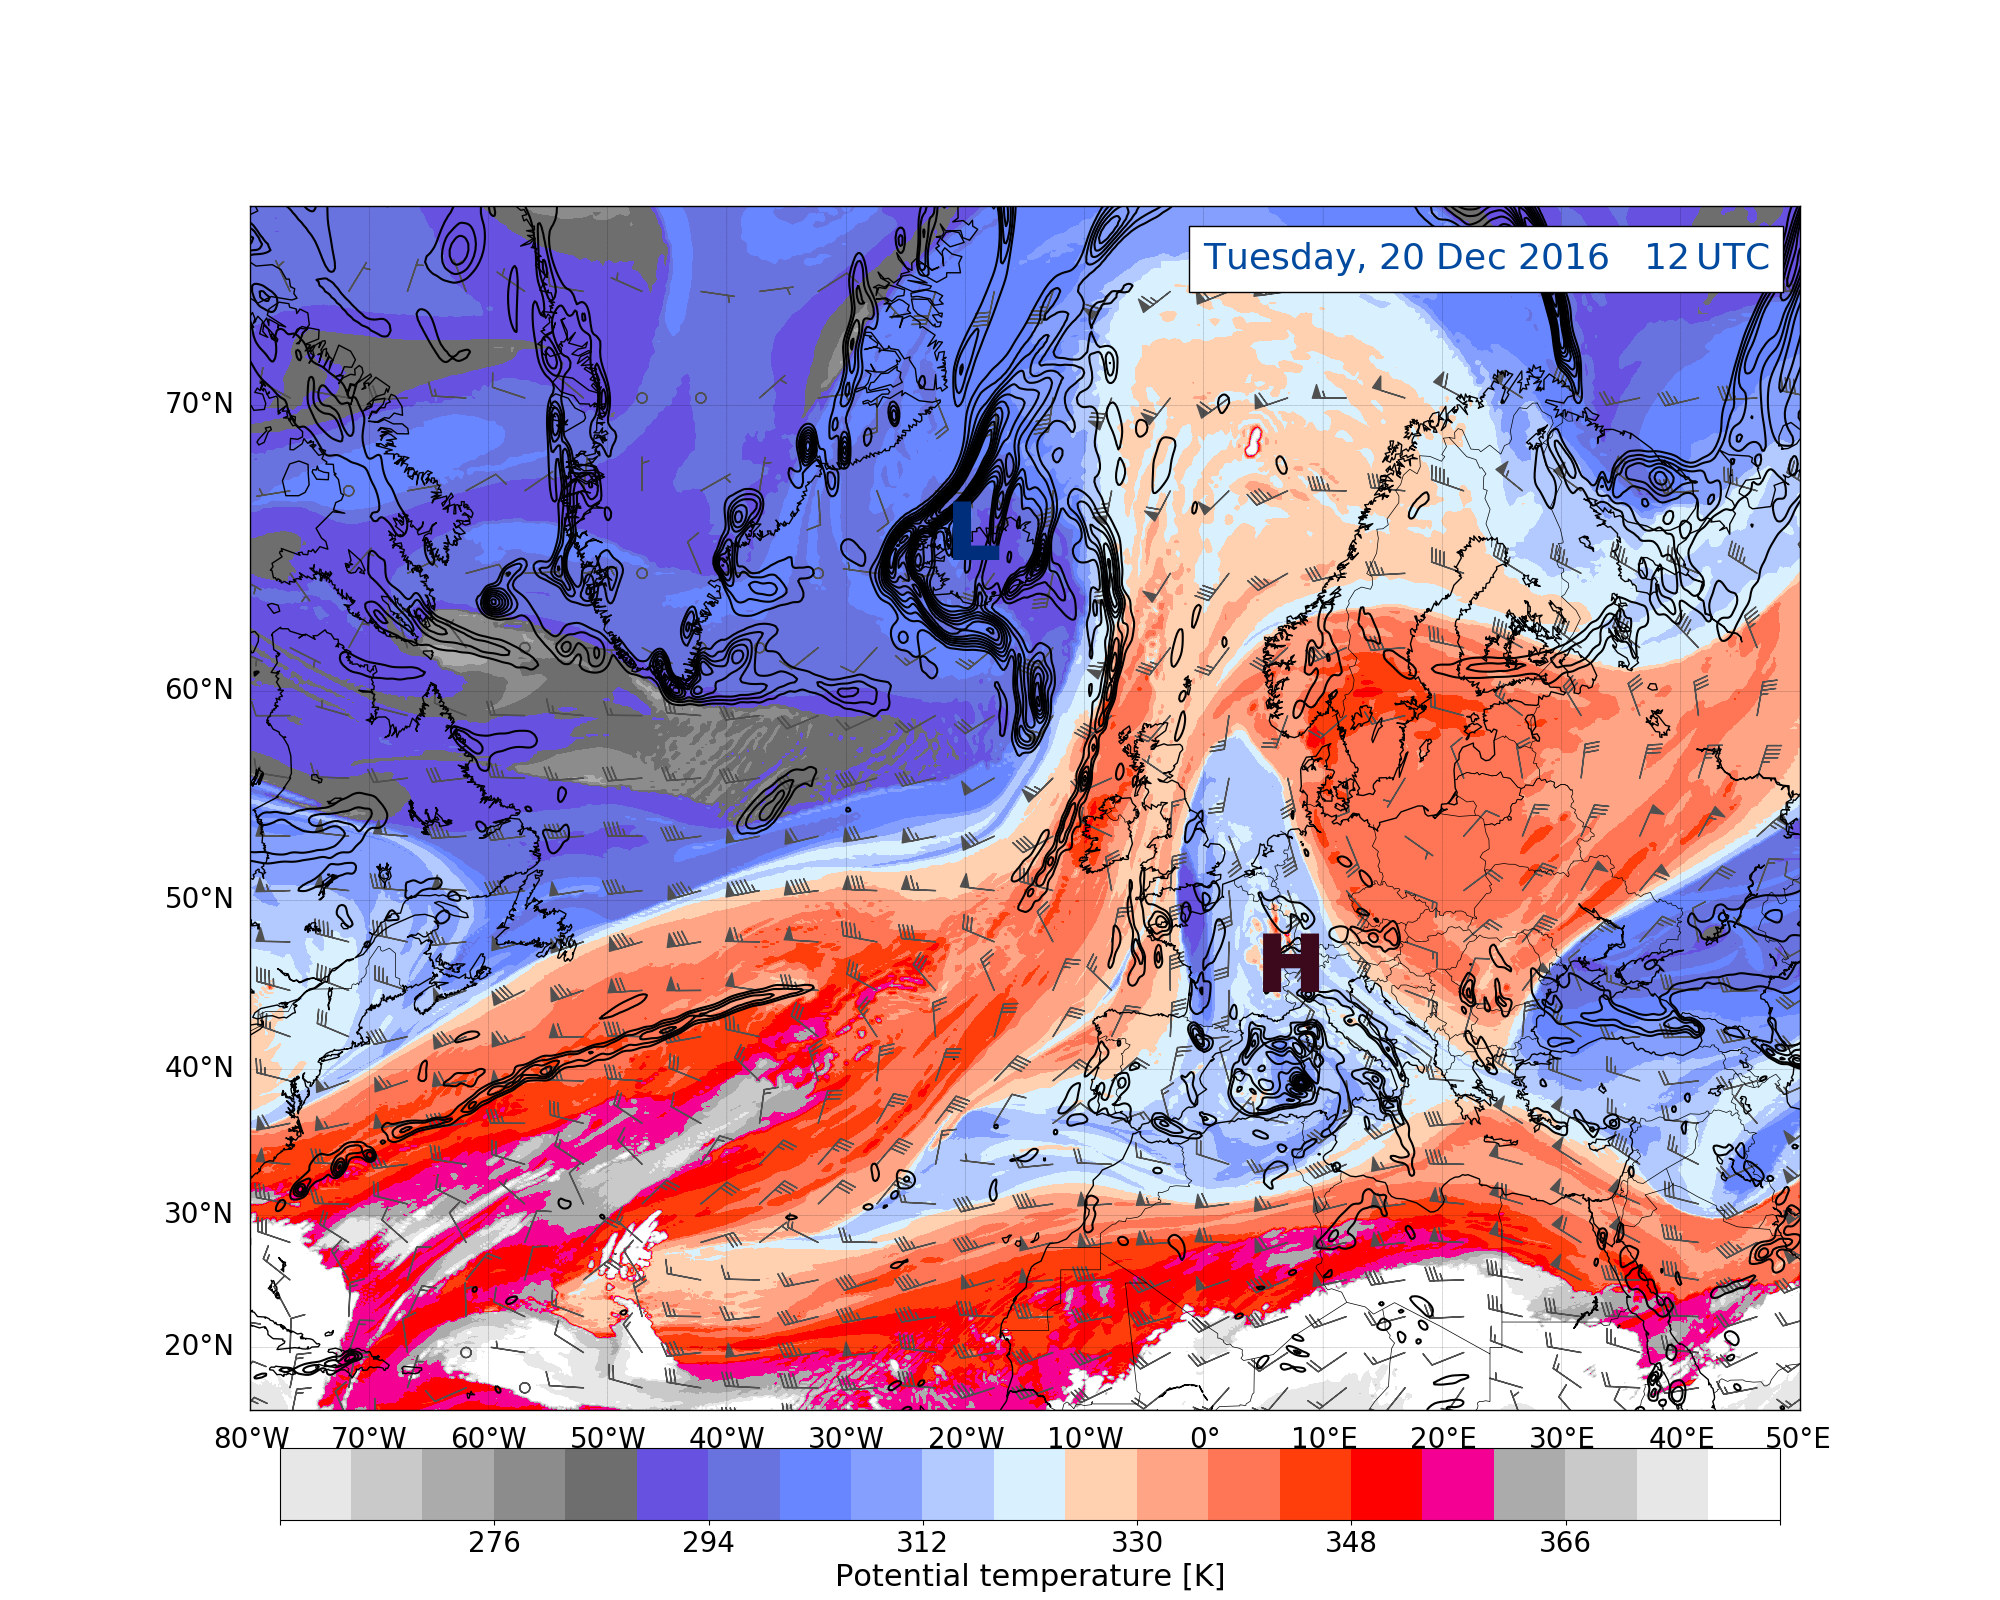
\includegraphics[trim={4.2cm 0cm 4.3cm 5.1cm},clip,
%         width=\textwidth]{./fig_DynTropo/20161220_12}
%         \caption{}
%     \end{subfigure}
%     %
%     \begin{subfigure}[b]{0.49\textwidth}
%     	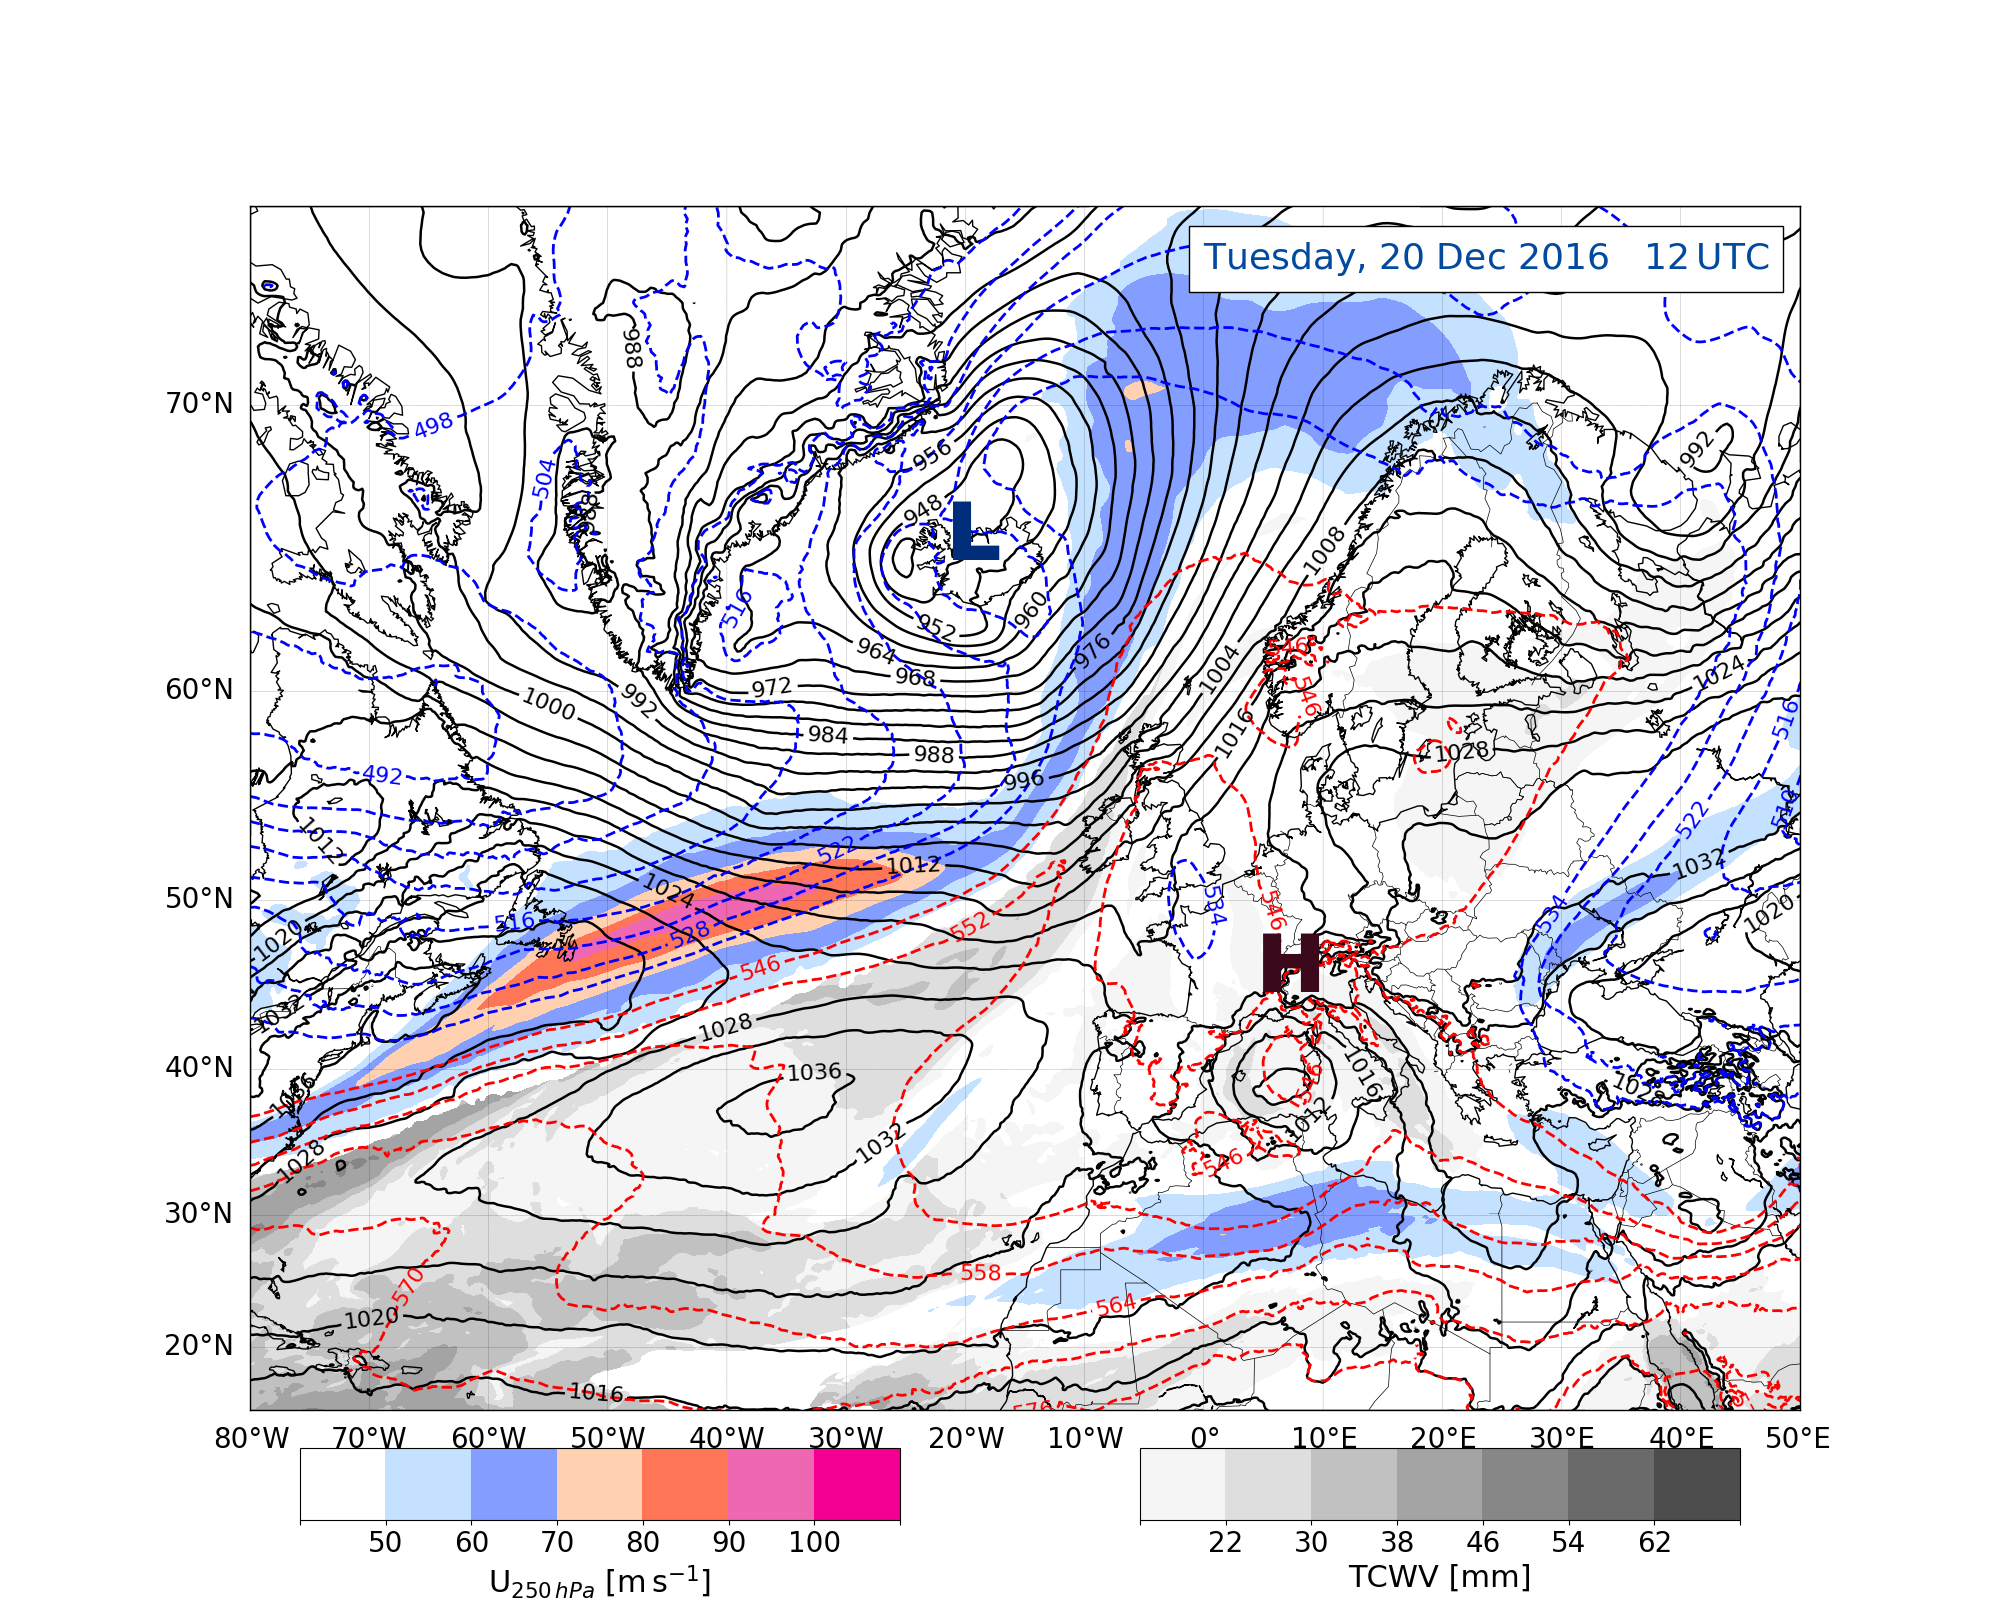
\includegraphics[trim={4.2cm 0cm 4.3cm 5.1cm},clip,
%          width=\textwidth]{./fig_Geopot_Jet/20161220_12}
%         \caption{}
%     \end{subfigure}
%     %
%     \begin{subfigure}[b]{0.49\textwidth}
%     	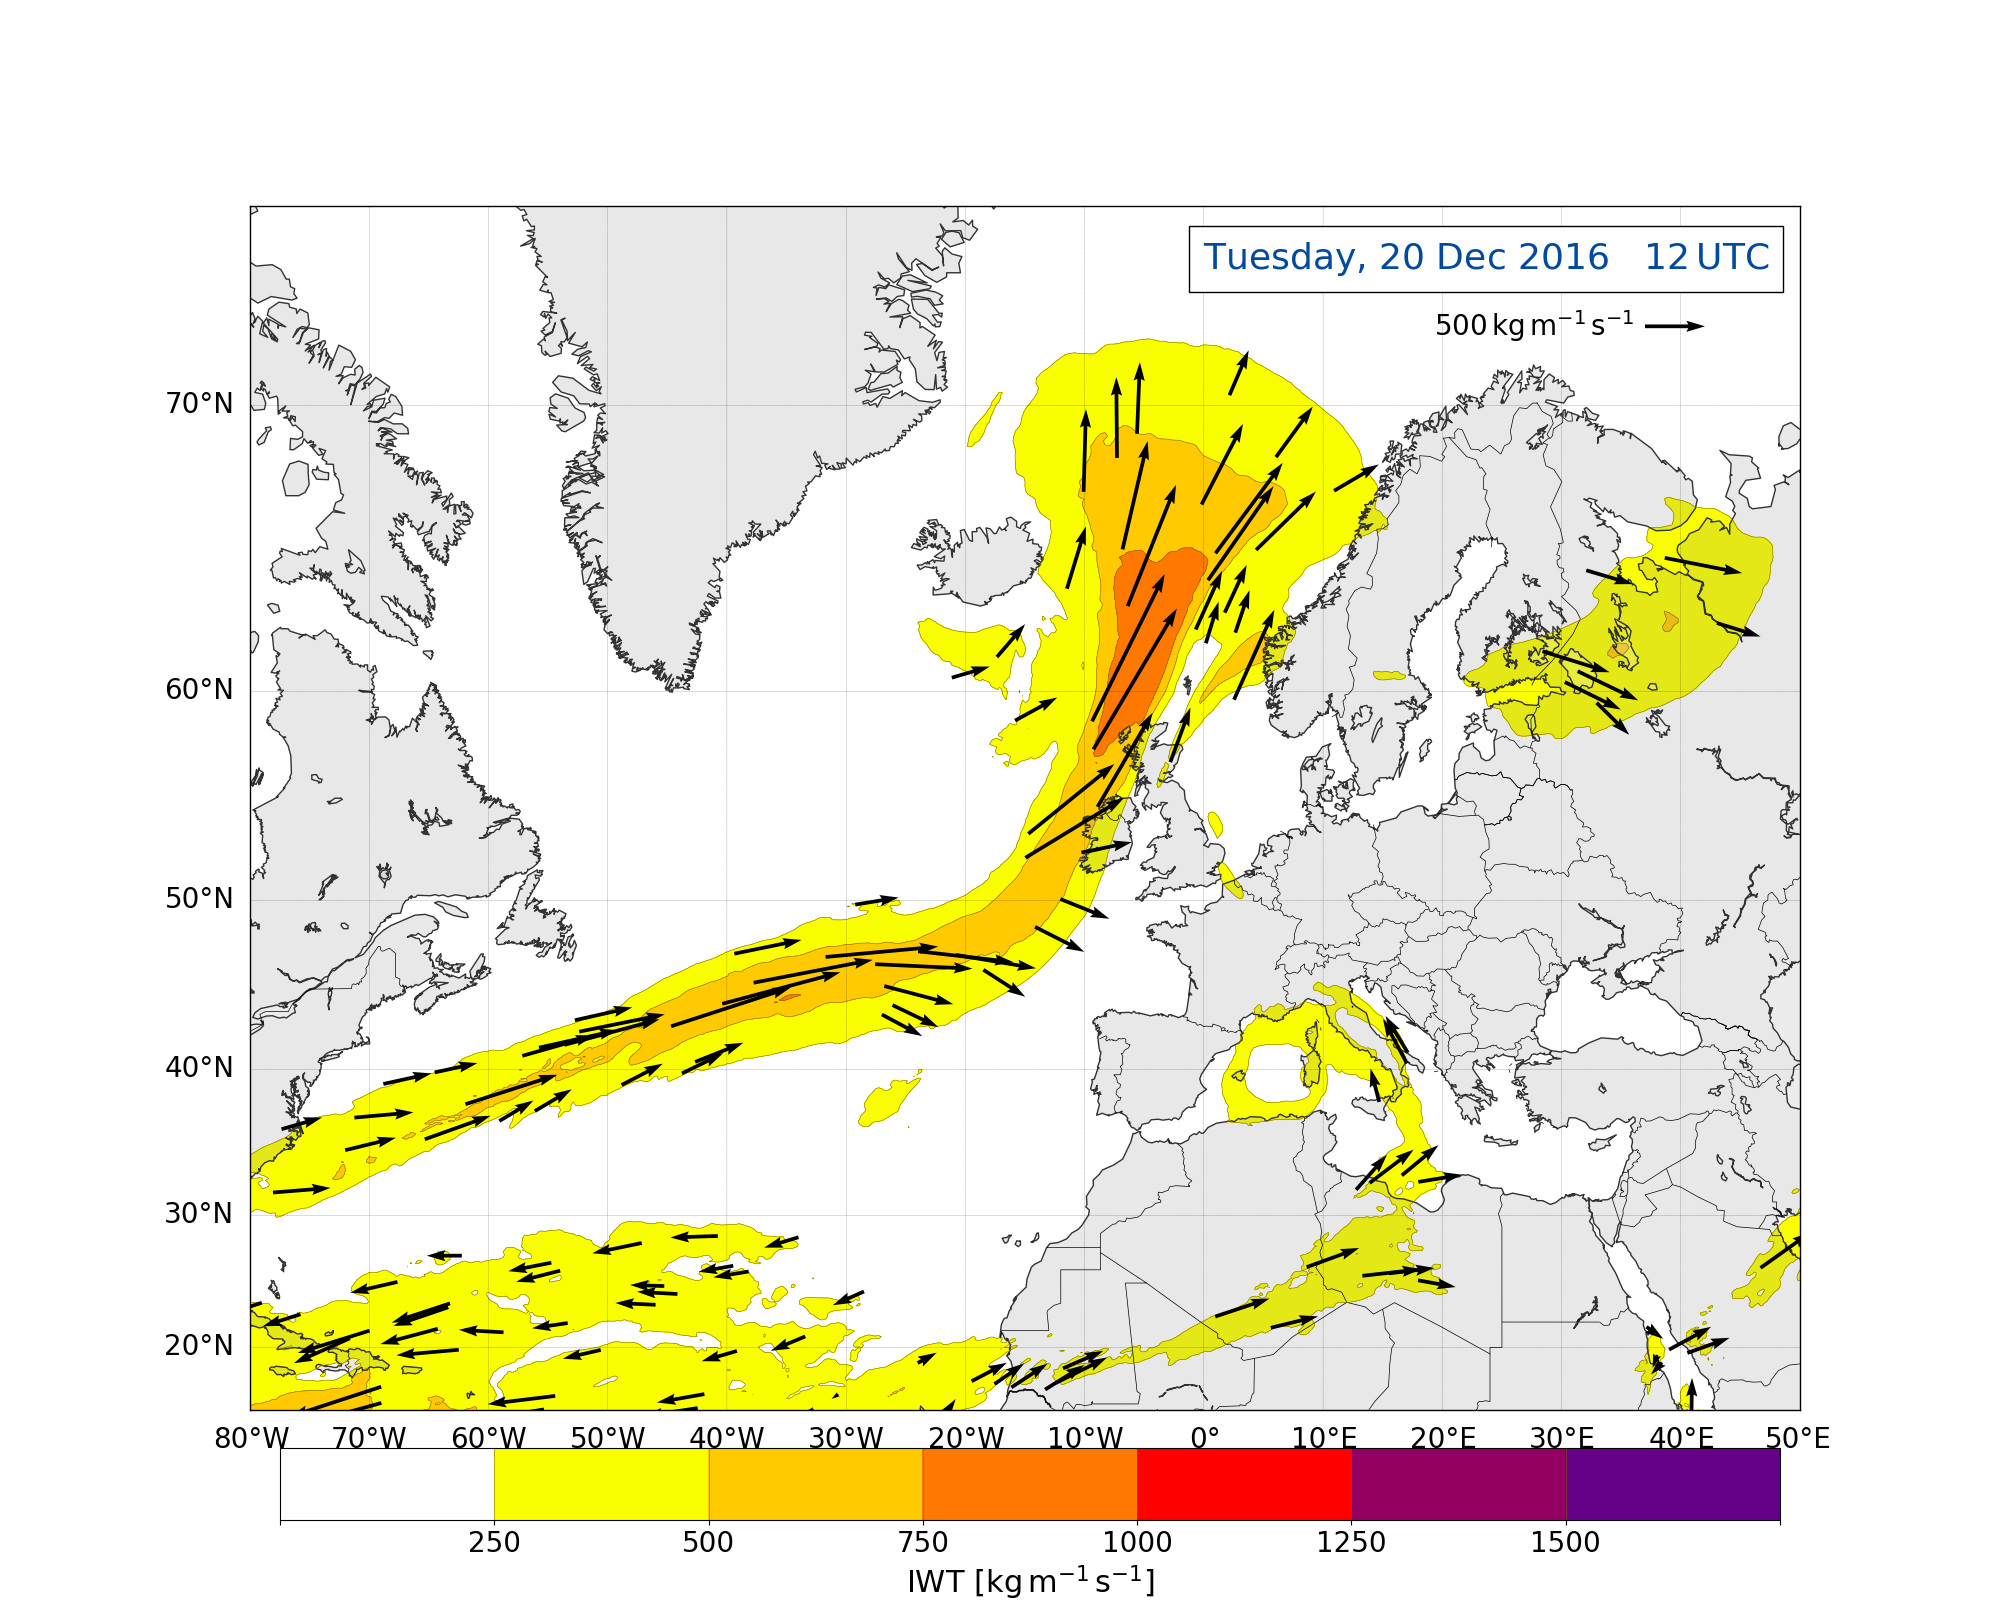
\includegraphics[trim={4.2cm 0cm 4.3cm 5.1cm},clip,
%          width=\textwidth]{./fig_Atm_Riv/20161220_12}
%         \caption{}
%     \end{subfigure}
%     %
%     \begin{subfigure}[b]{0.49\textwidth}
%     	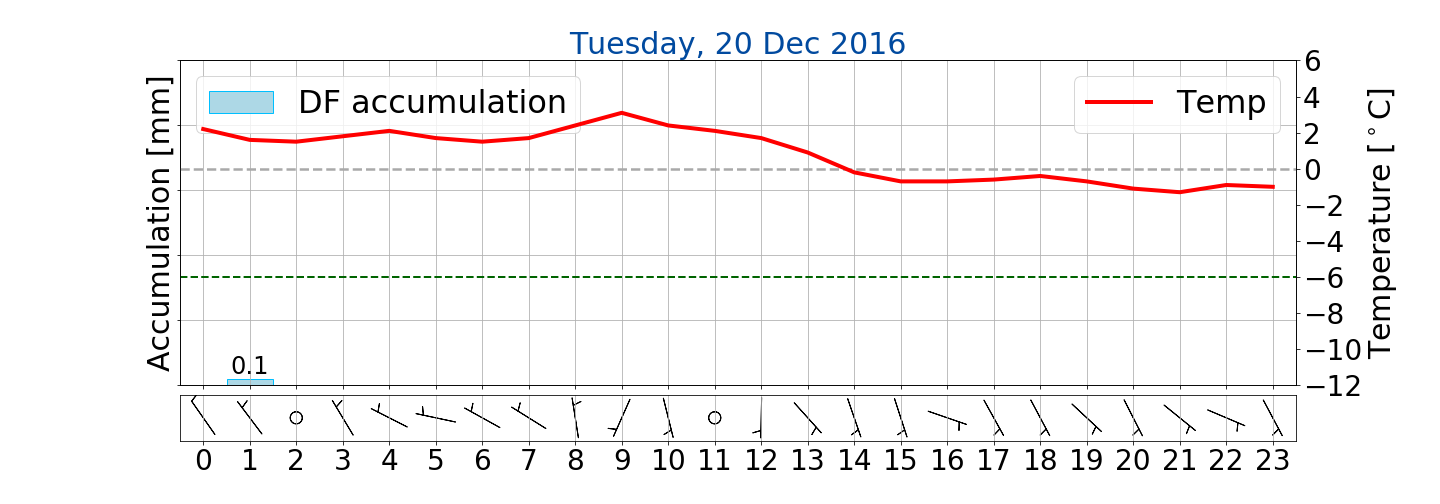
\includegraphics[trim={4.9cm 1.cm 1.5cm 1cm},clip,
% 		width=\textwidth]{./fig_weathermast/T_P_U_20161220}
%         \caption{}
%     \end{subfigure}
% \end{figure}


% %%% Dynamic tropopause map %%%%%%%%%%%%%%%%%%%%%%%%%%%%%%%%%%%%%
% % !TeX spellcheck = en_GB
\begin{figure}[h!]
    \centering
%%%%%% 20/12
    \begin{subfigure}[b]{0.49\textwidth}
        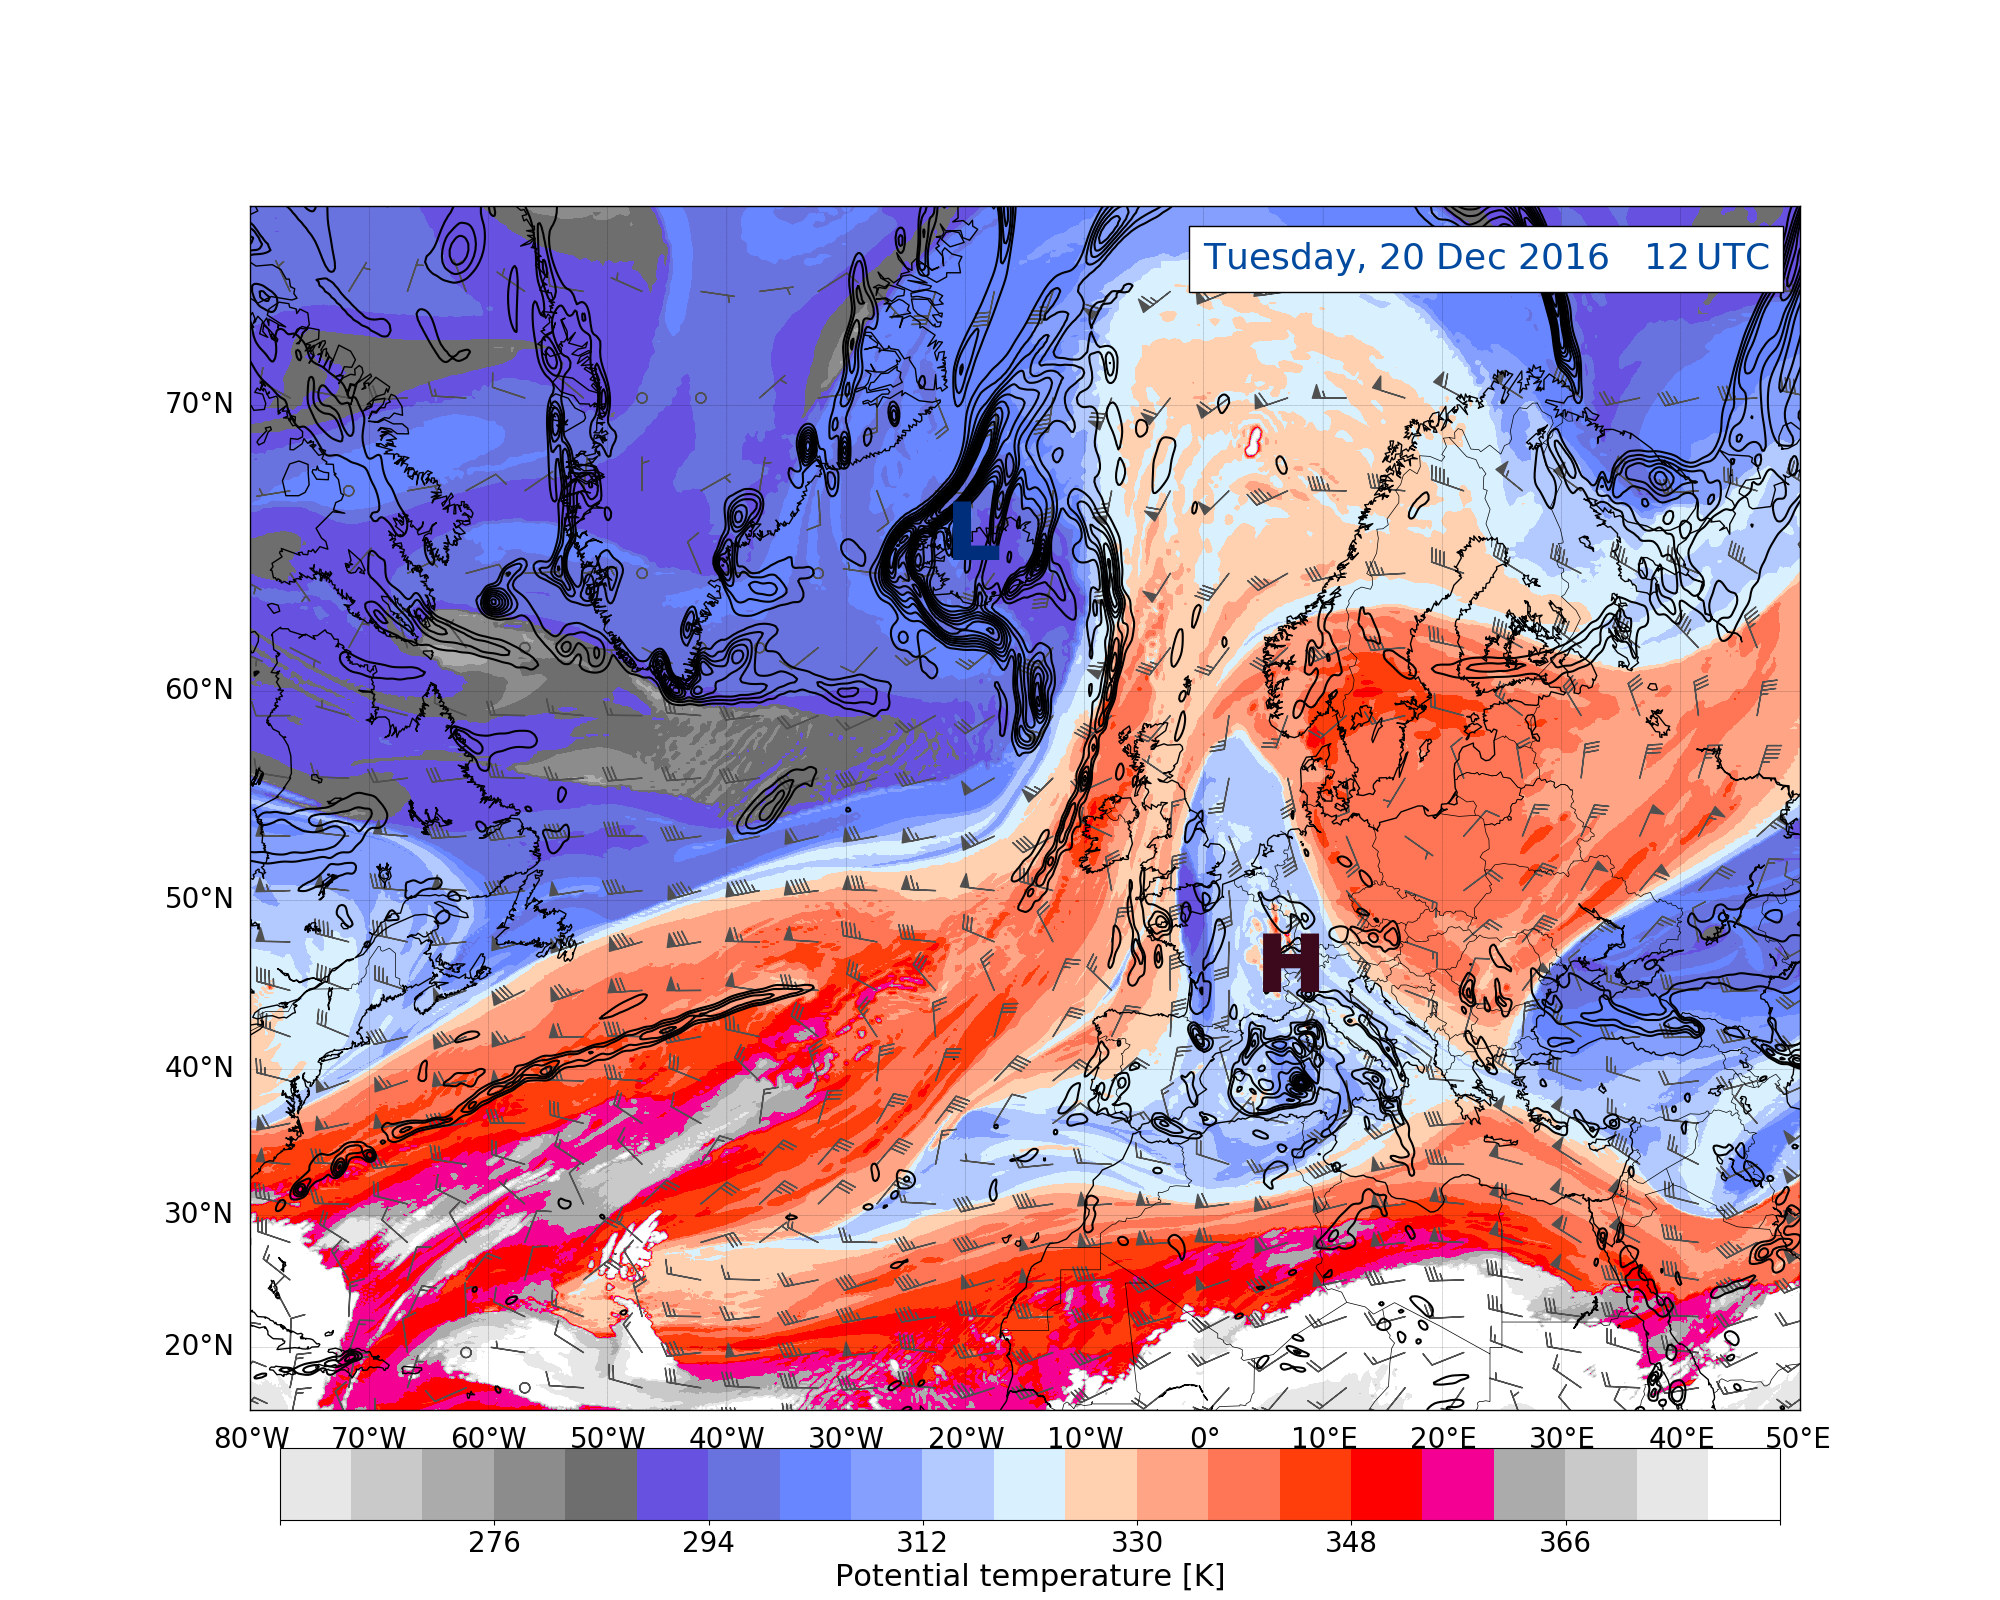
\includegraphics[trim={4.2cm 3.9cm 4.3cm 5.1cm},clip,
        width=\textwidth]{./fig_DynTropo/20161220_12}
        \caption{} \label{fig:DT20}
    \end{subfigure}
%%%%%% 21/12
    \begin{subfigure}[b]{0.49\textwidth}
        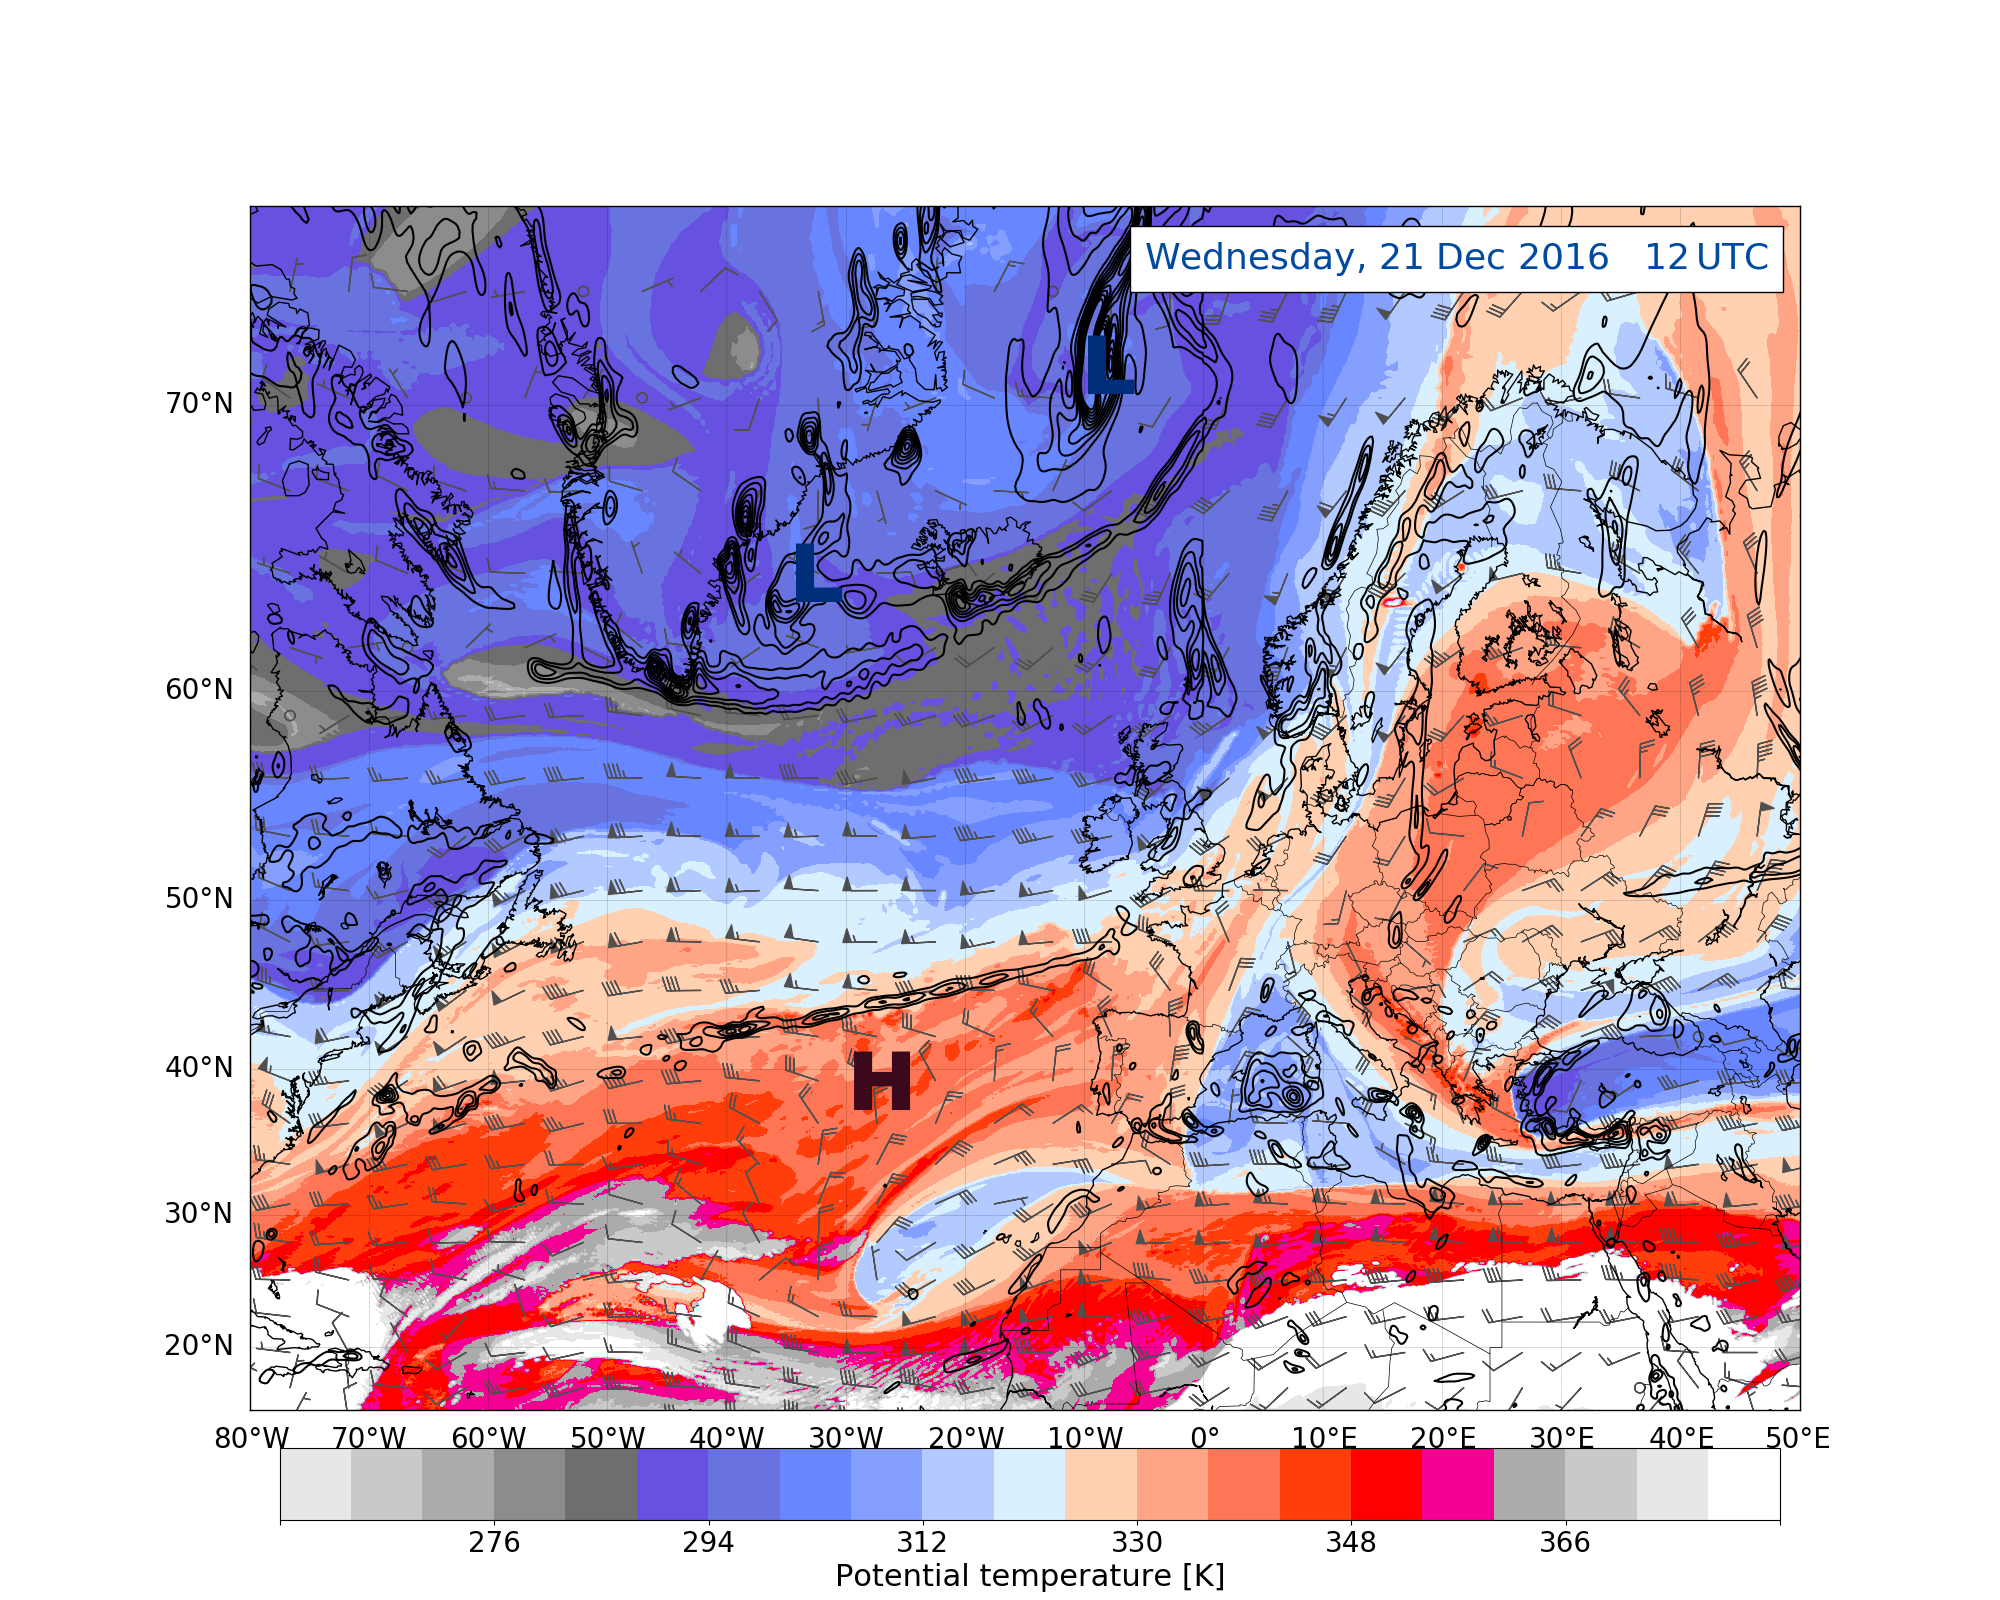
\includegraphics[trim={4.2cm 3.9cm 4.3cm 5.1cm},clip,
        width=\textwidth]{./fig_DynTropo/20161221_12}
        \caption{}\label{fig:DT21}
    \end{subfigure}

%%%%%% 22/12
\begin{subfigure}[b]{0.49\textwidth}
	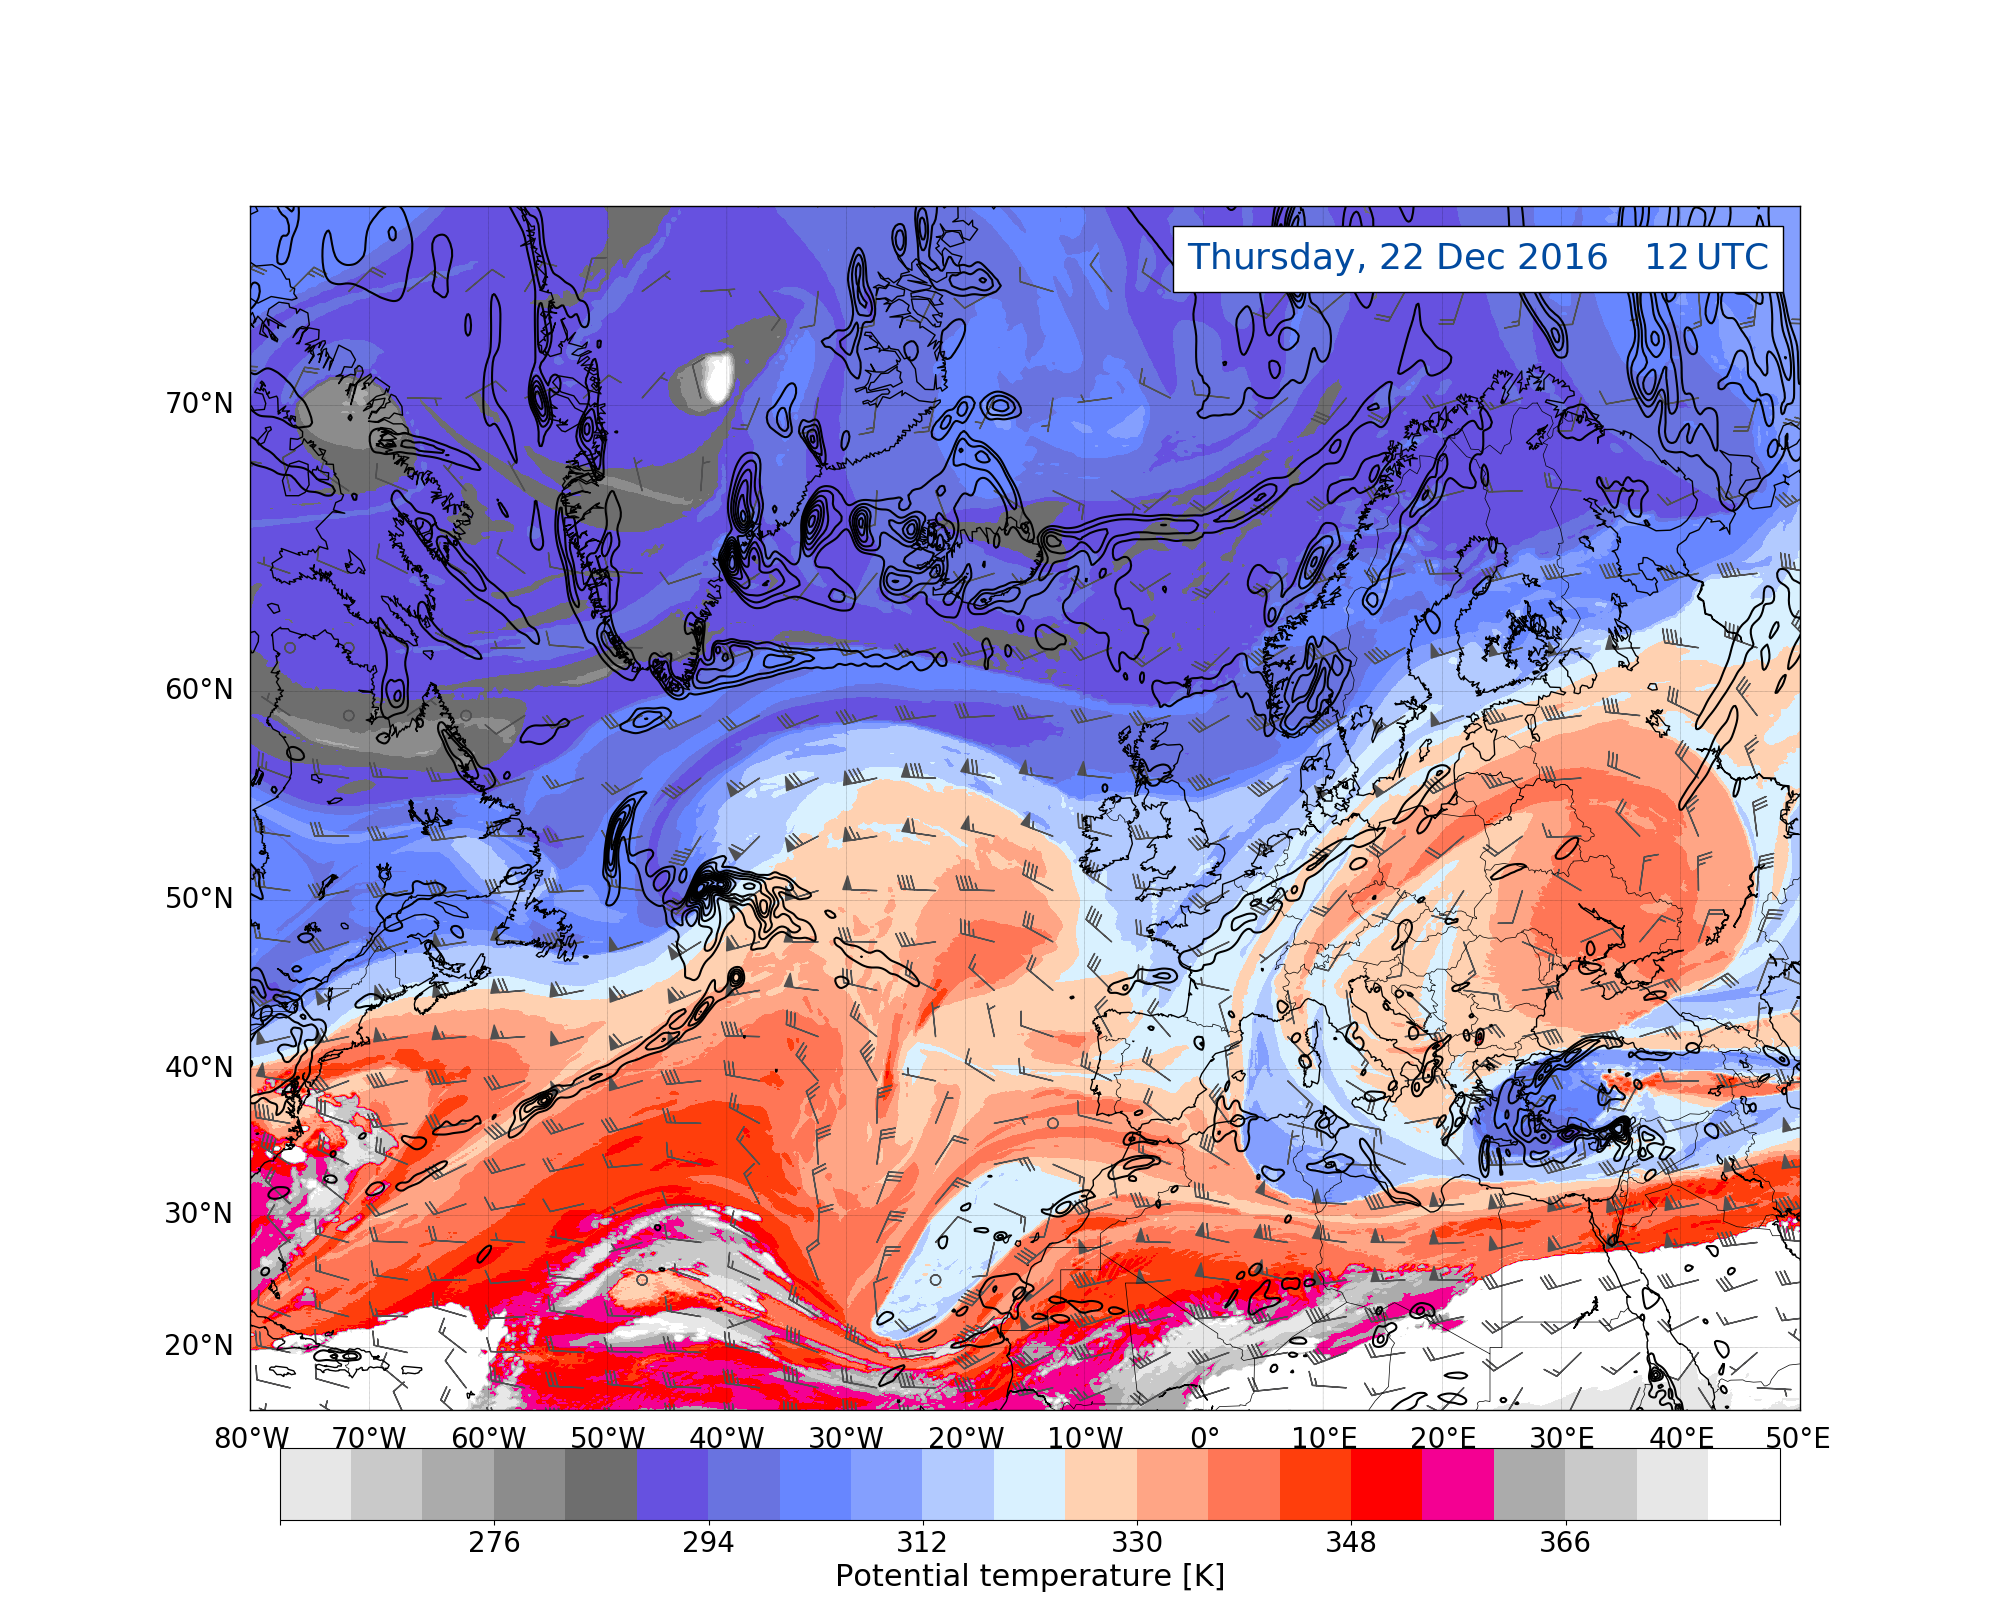
\includegraphics[trim={4.2cm 3.9cm 4.3cm 5.1cm},clip,
	width=\textwidth]{./fig_DynTropo/20161222_12}
	\caption{}\label{fig:DT22}
\end{subfigure}
%%%%%% 23/12
\begin{subfigure}[b]{0.49\textwidth}
	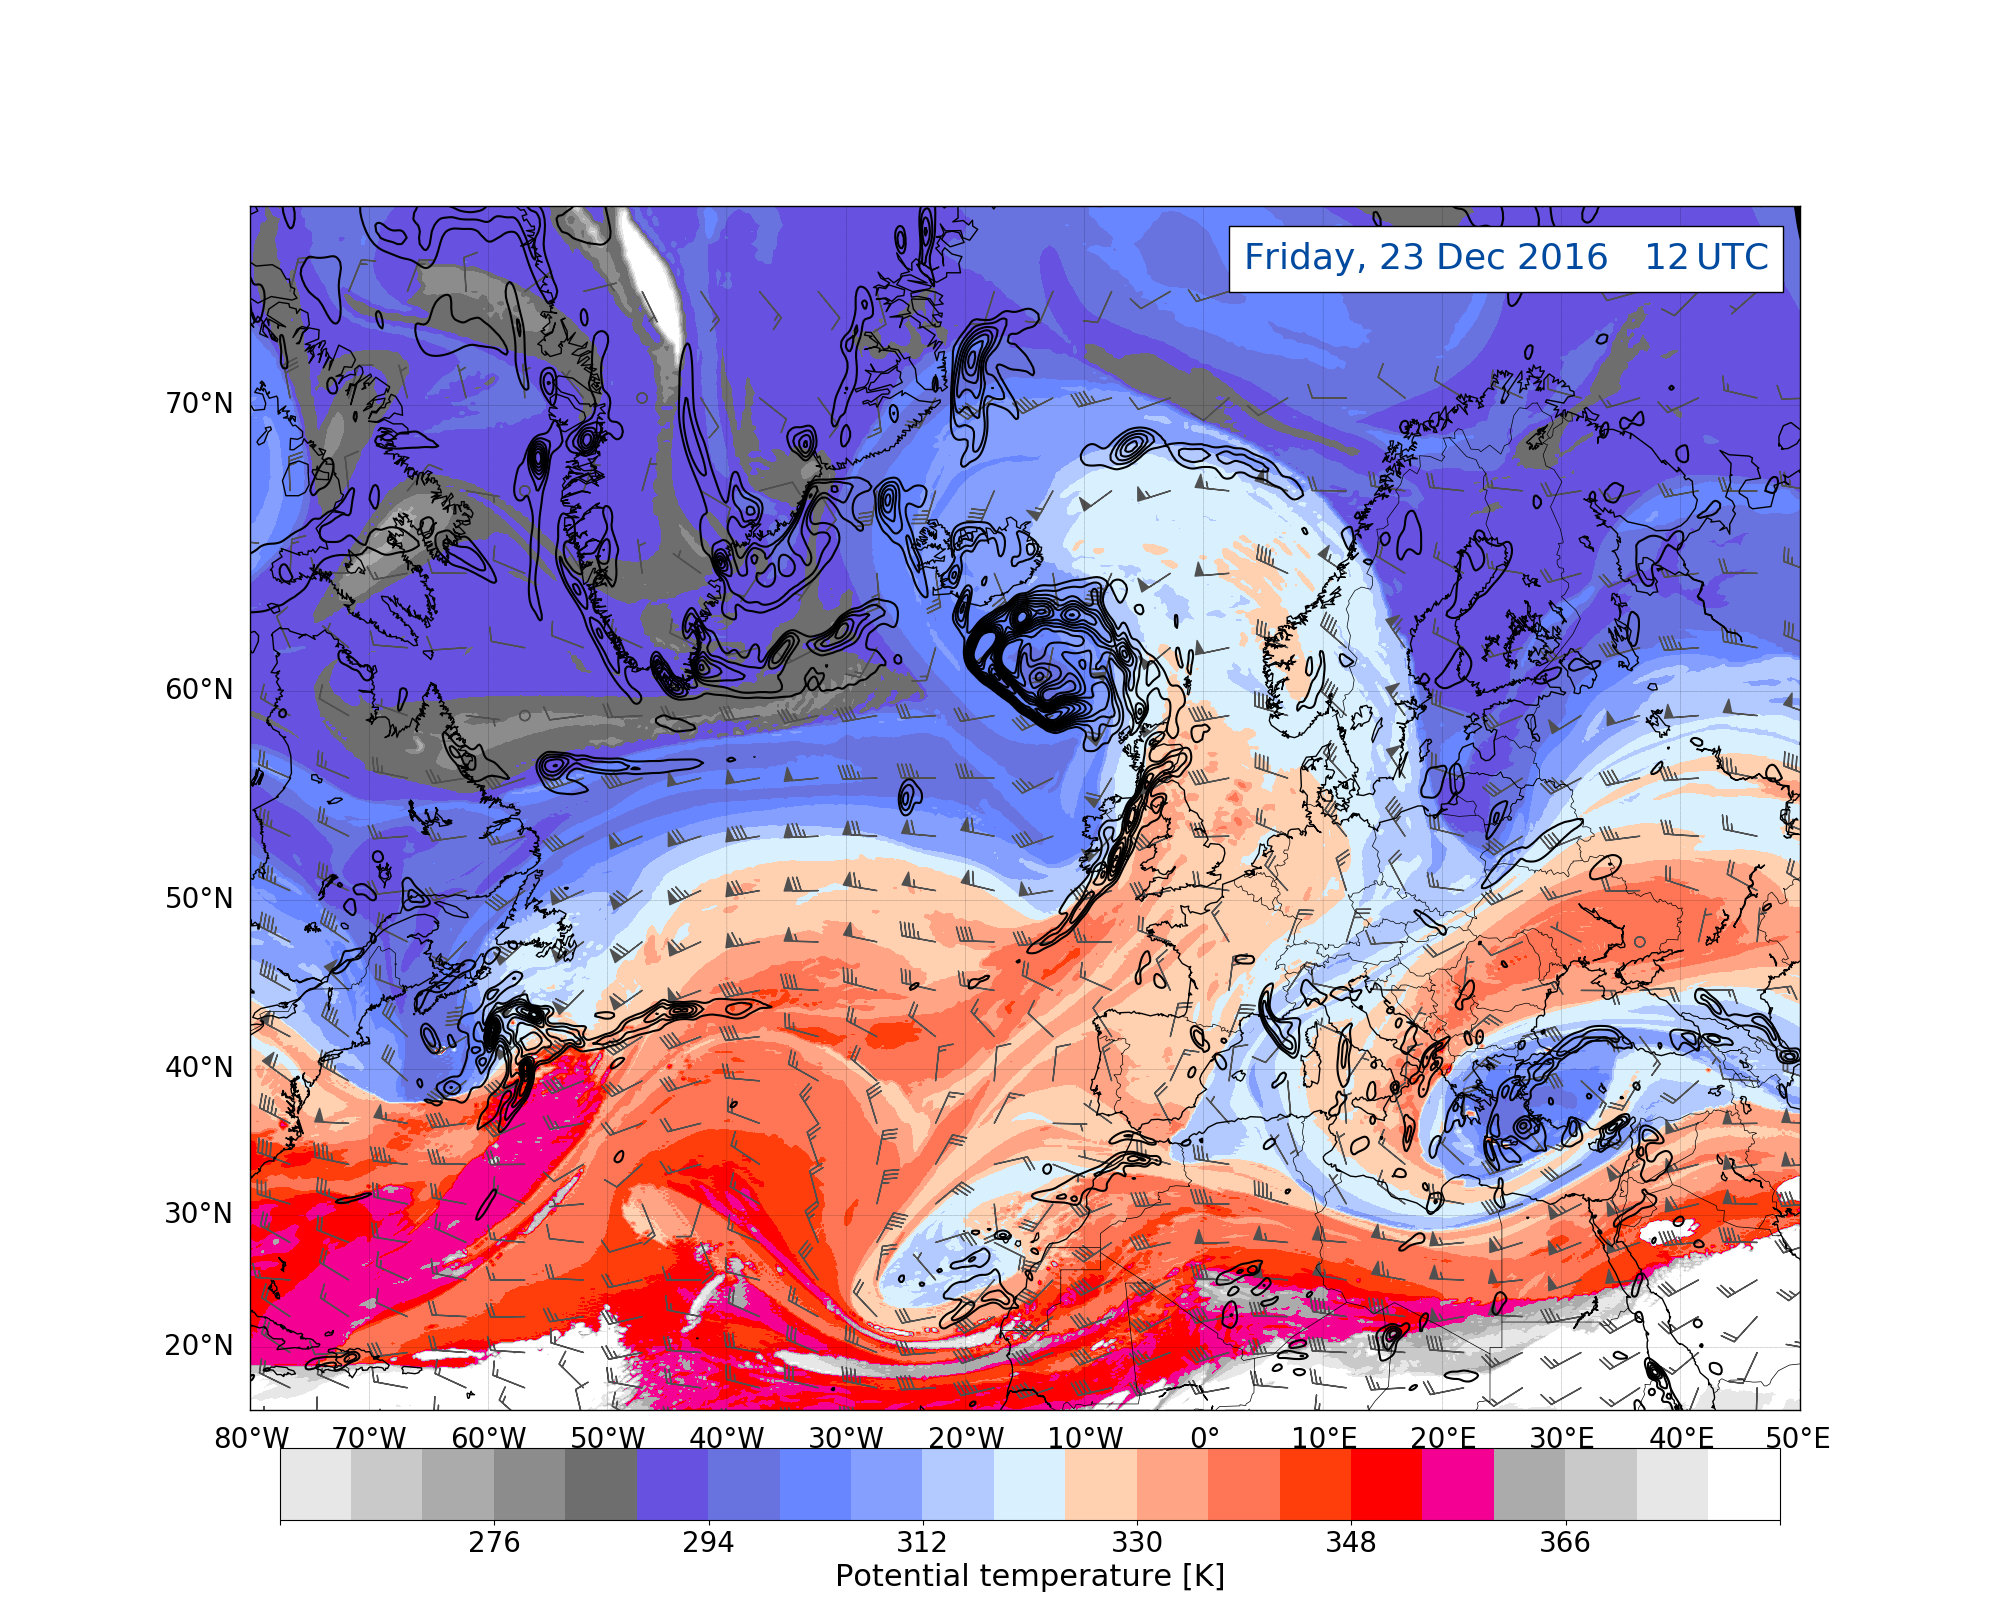
\includegraphics[trim={4.2cm 3.9cm 4.3cm 5.1cm},clip,
	width=\textwidth]{./fig_DynTropo/20161223_12}
	\caption{}\label{fig:DT23}
\end{subfigure}

%%%%%% label
    \begin{subfigure}[b]{\textwidth}
        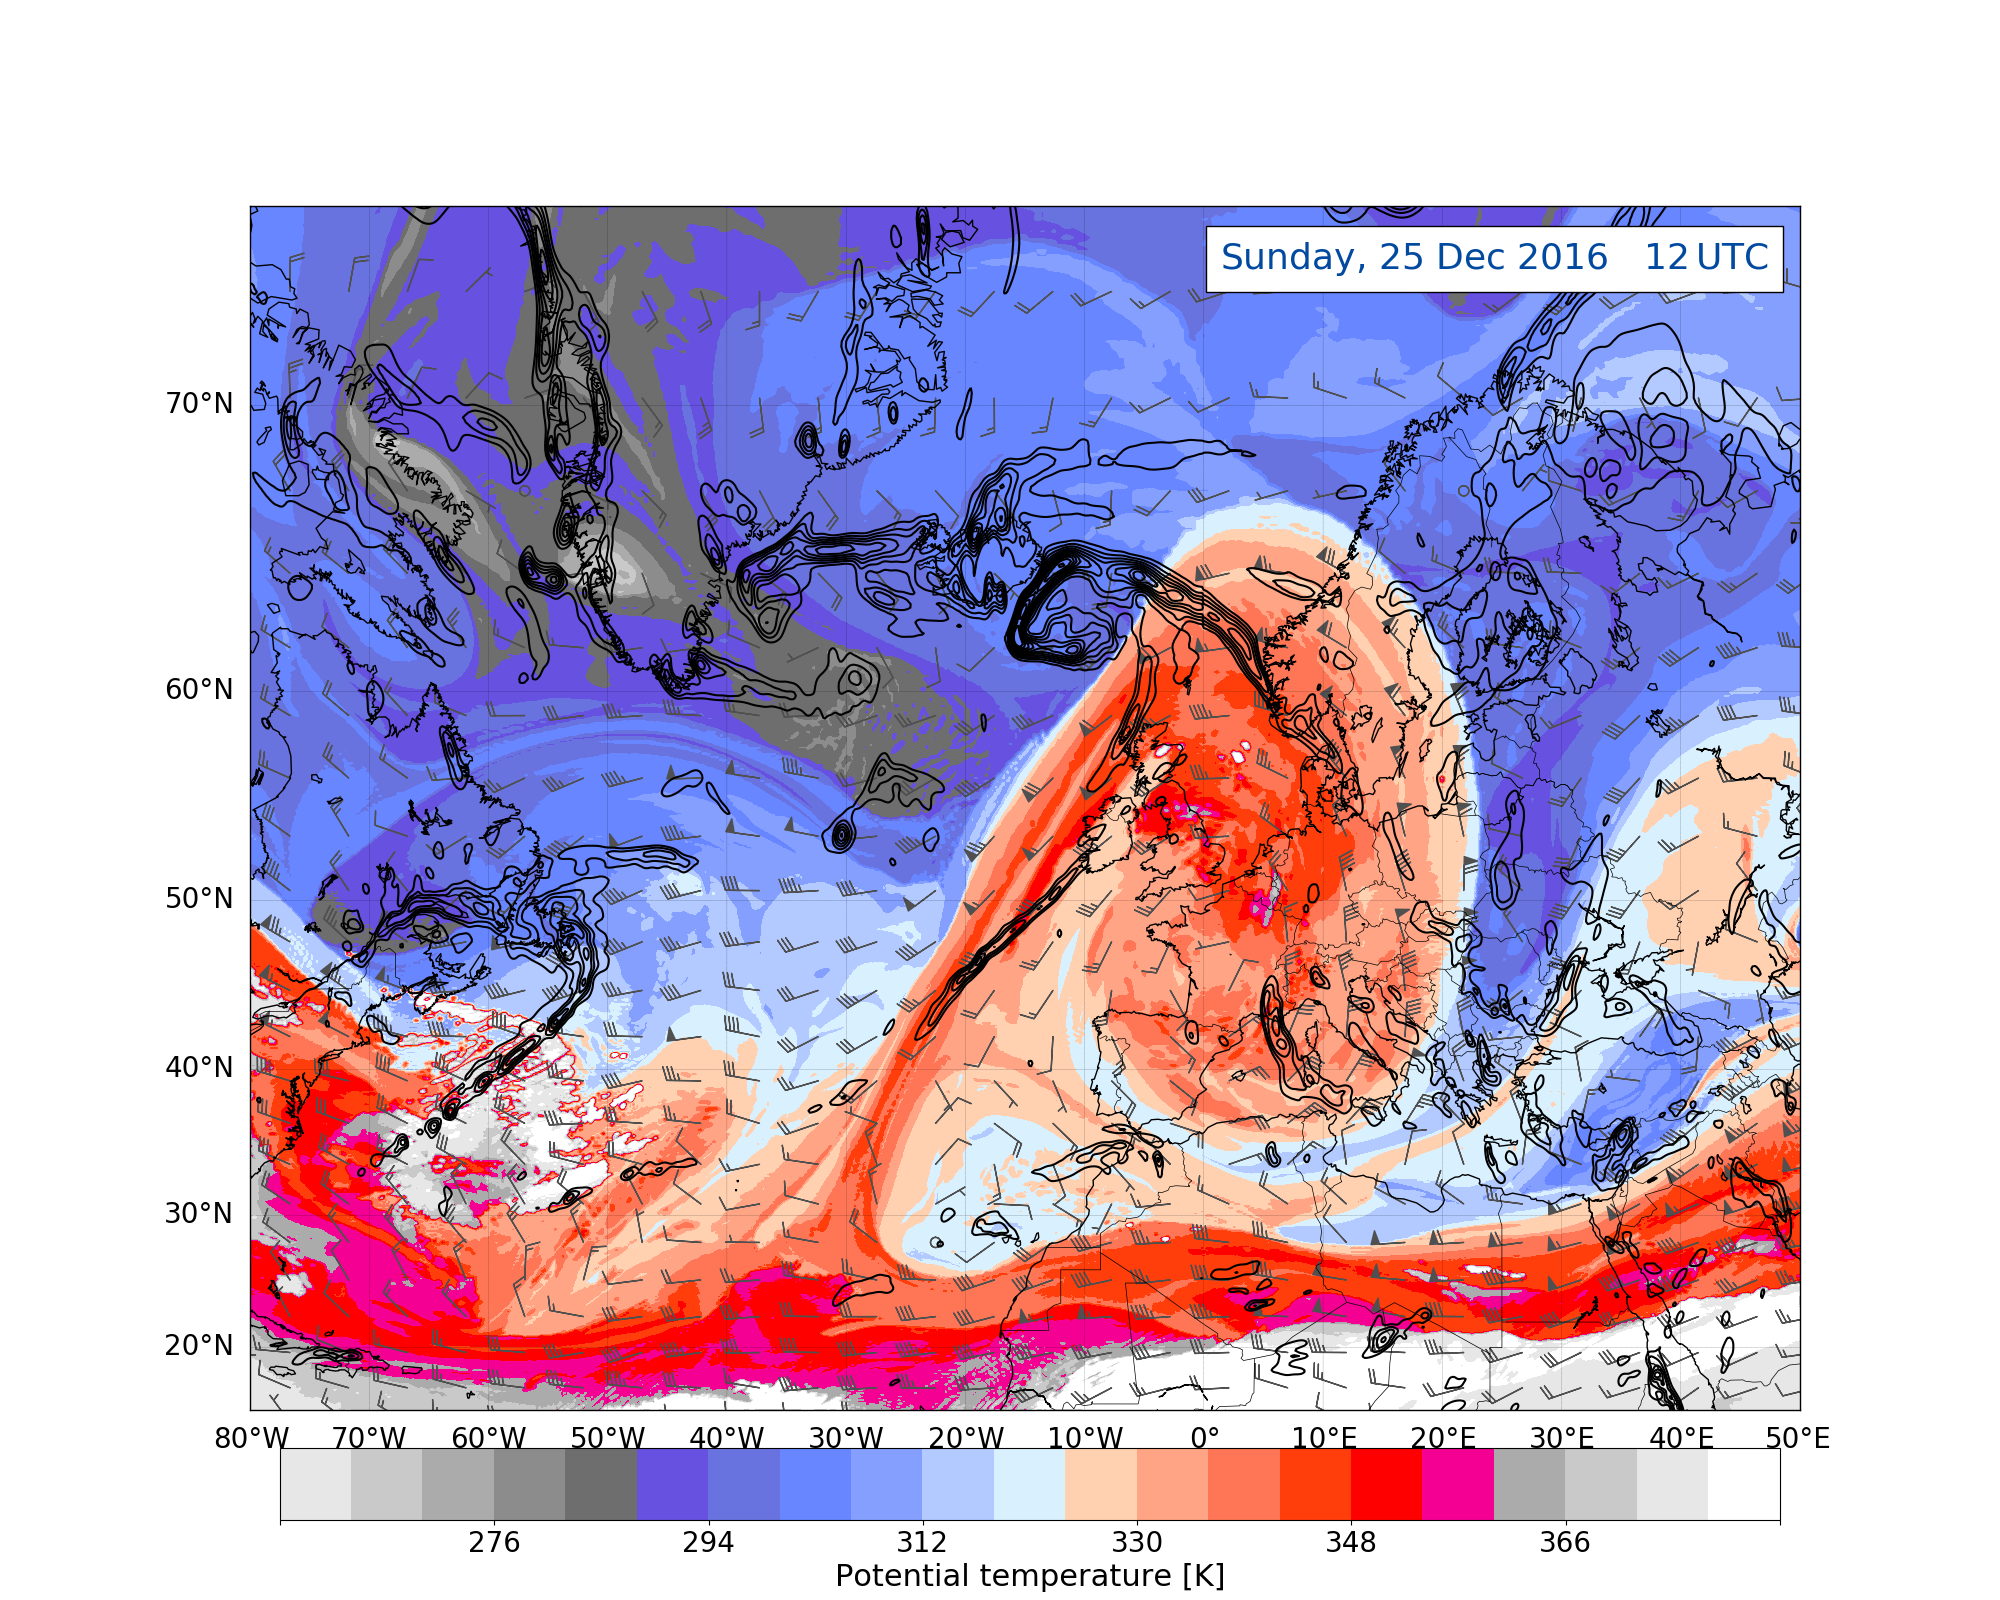
\includegraphics[trim={4.2cm 0cm 4.3cm 36.8cm},clip,
        width=\textwidth]{./fig_DynTropo/20161225_12}
    \end{subfigure}
\end{figure}
%
\begin{figure}\ContinuedFloat
	\centering
%%%%%% 24/12
    \begin{subfigure}[b]{0.49\textwidth}
        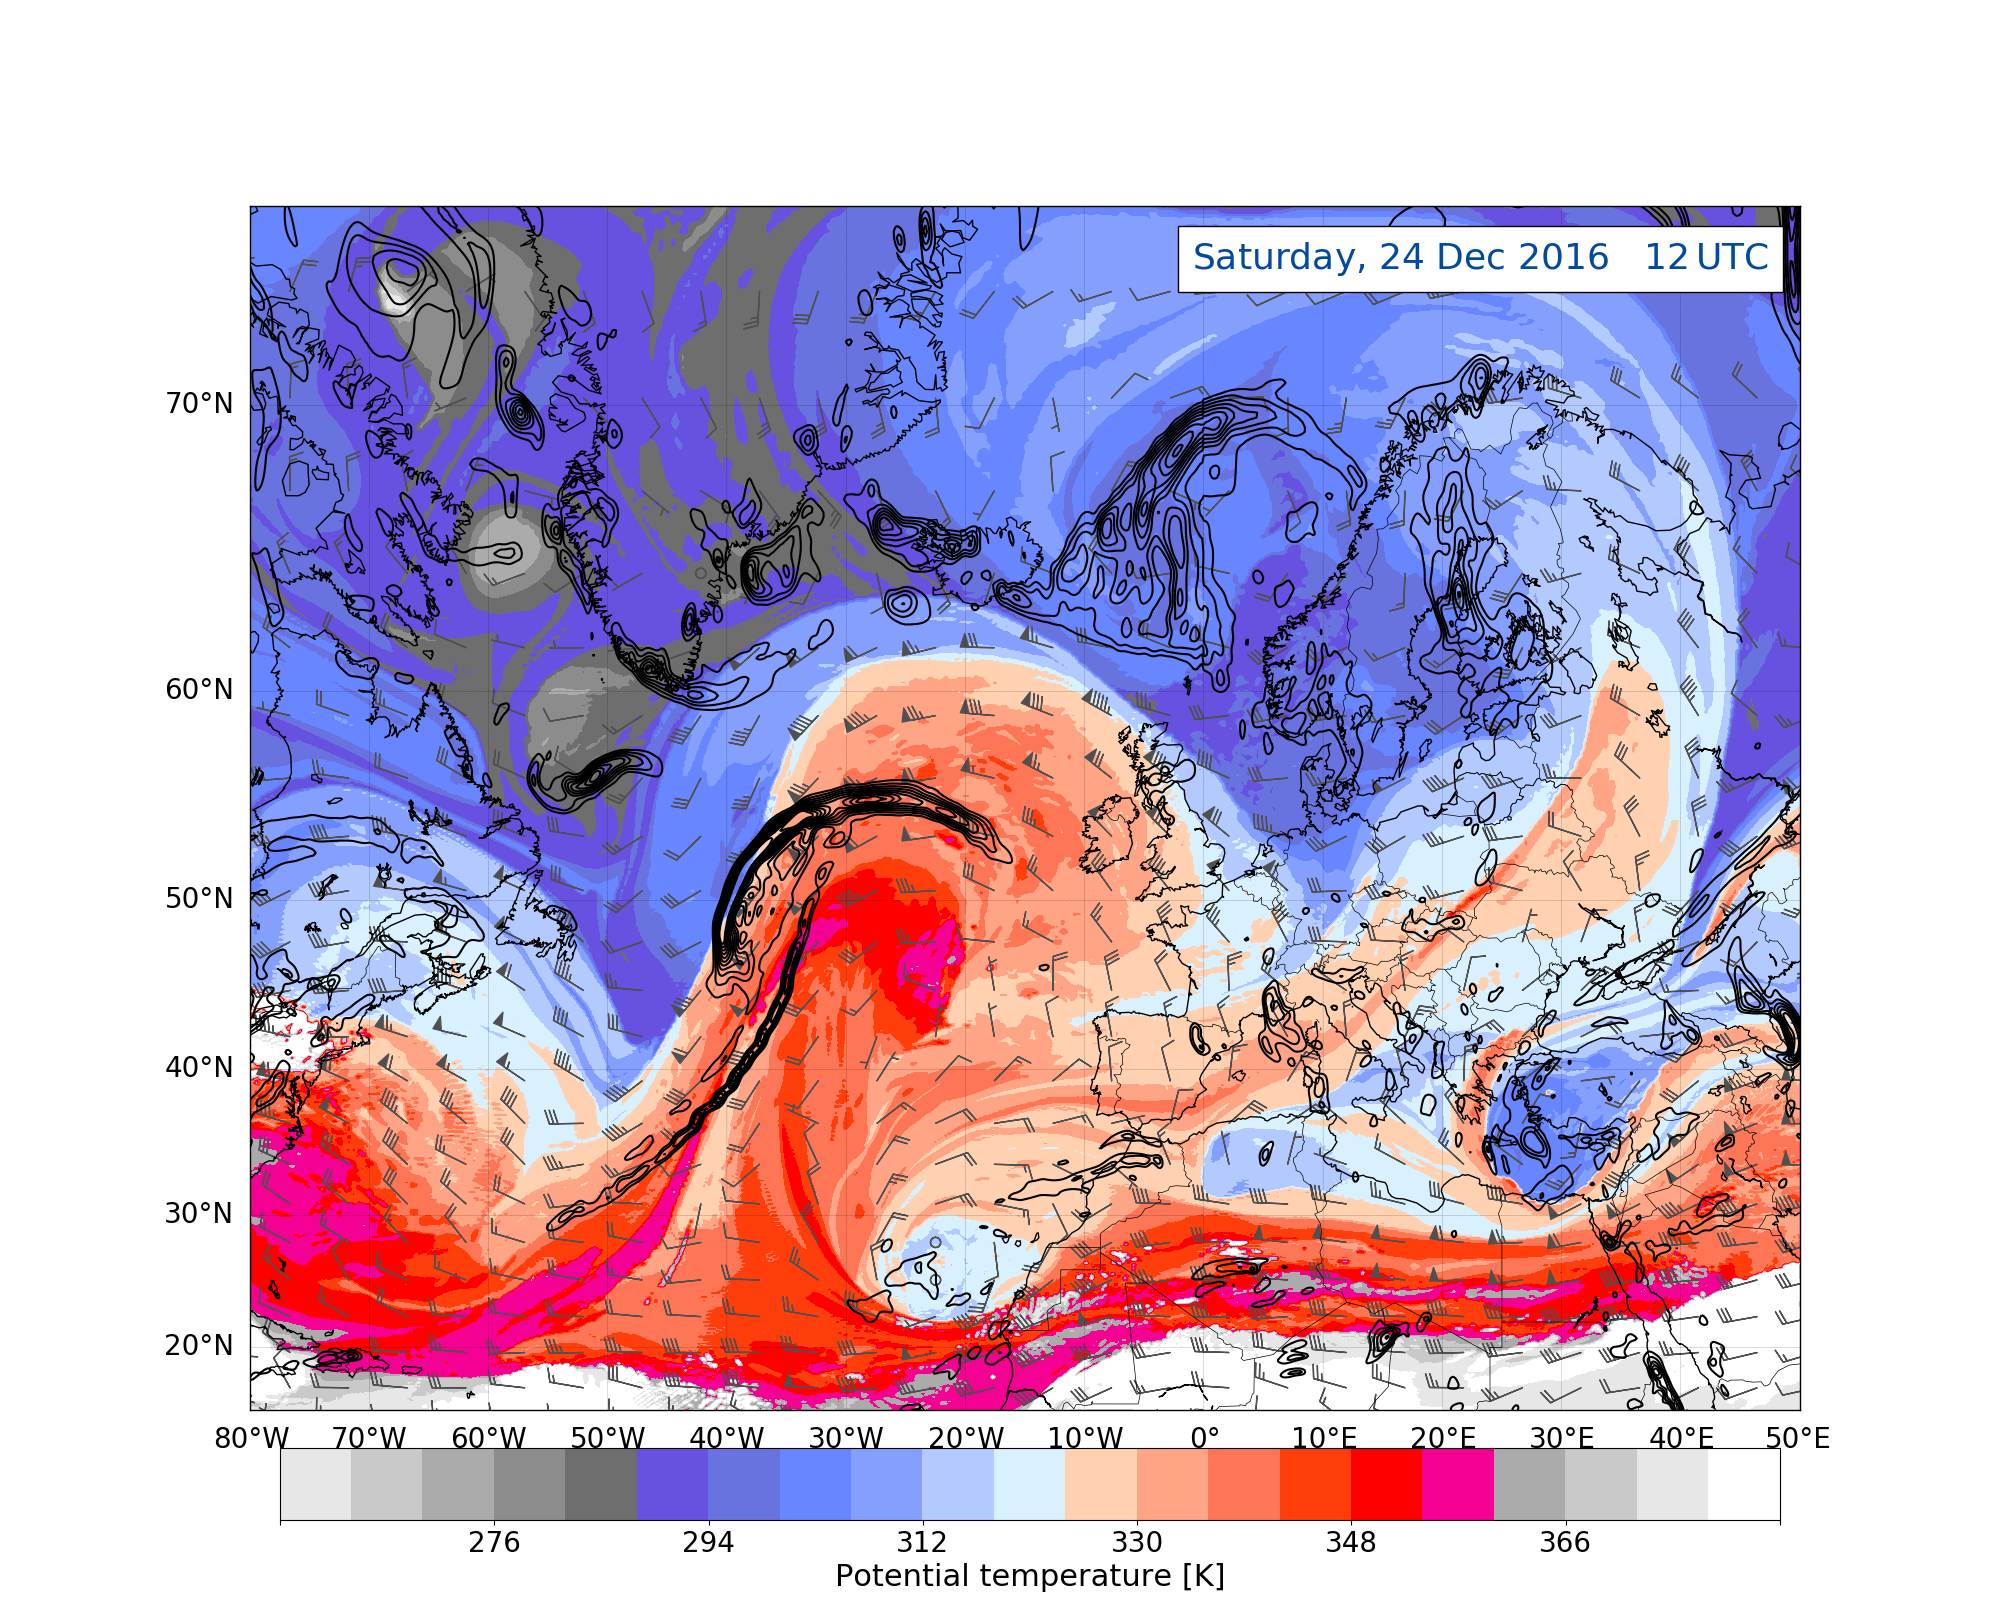
\includegraphics[trim={4.2cm 3.9cm 4.3cm 5.1cm},clip,
        width=\textwidth]{./fig_DynTropo/20161224_12}
        \caption{}\label{fig:DT24}
    \end{subfigure}
%%%%%% 25/12
    \begin{subfigure}[b]{0.49\textwidth}
        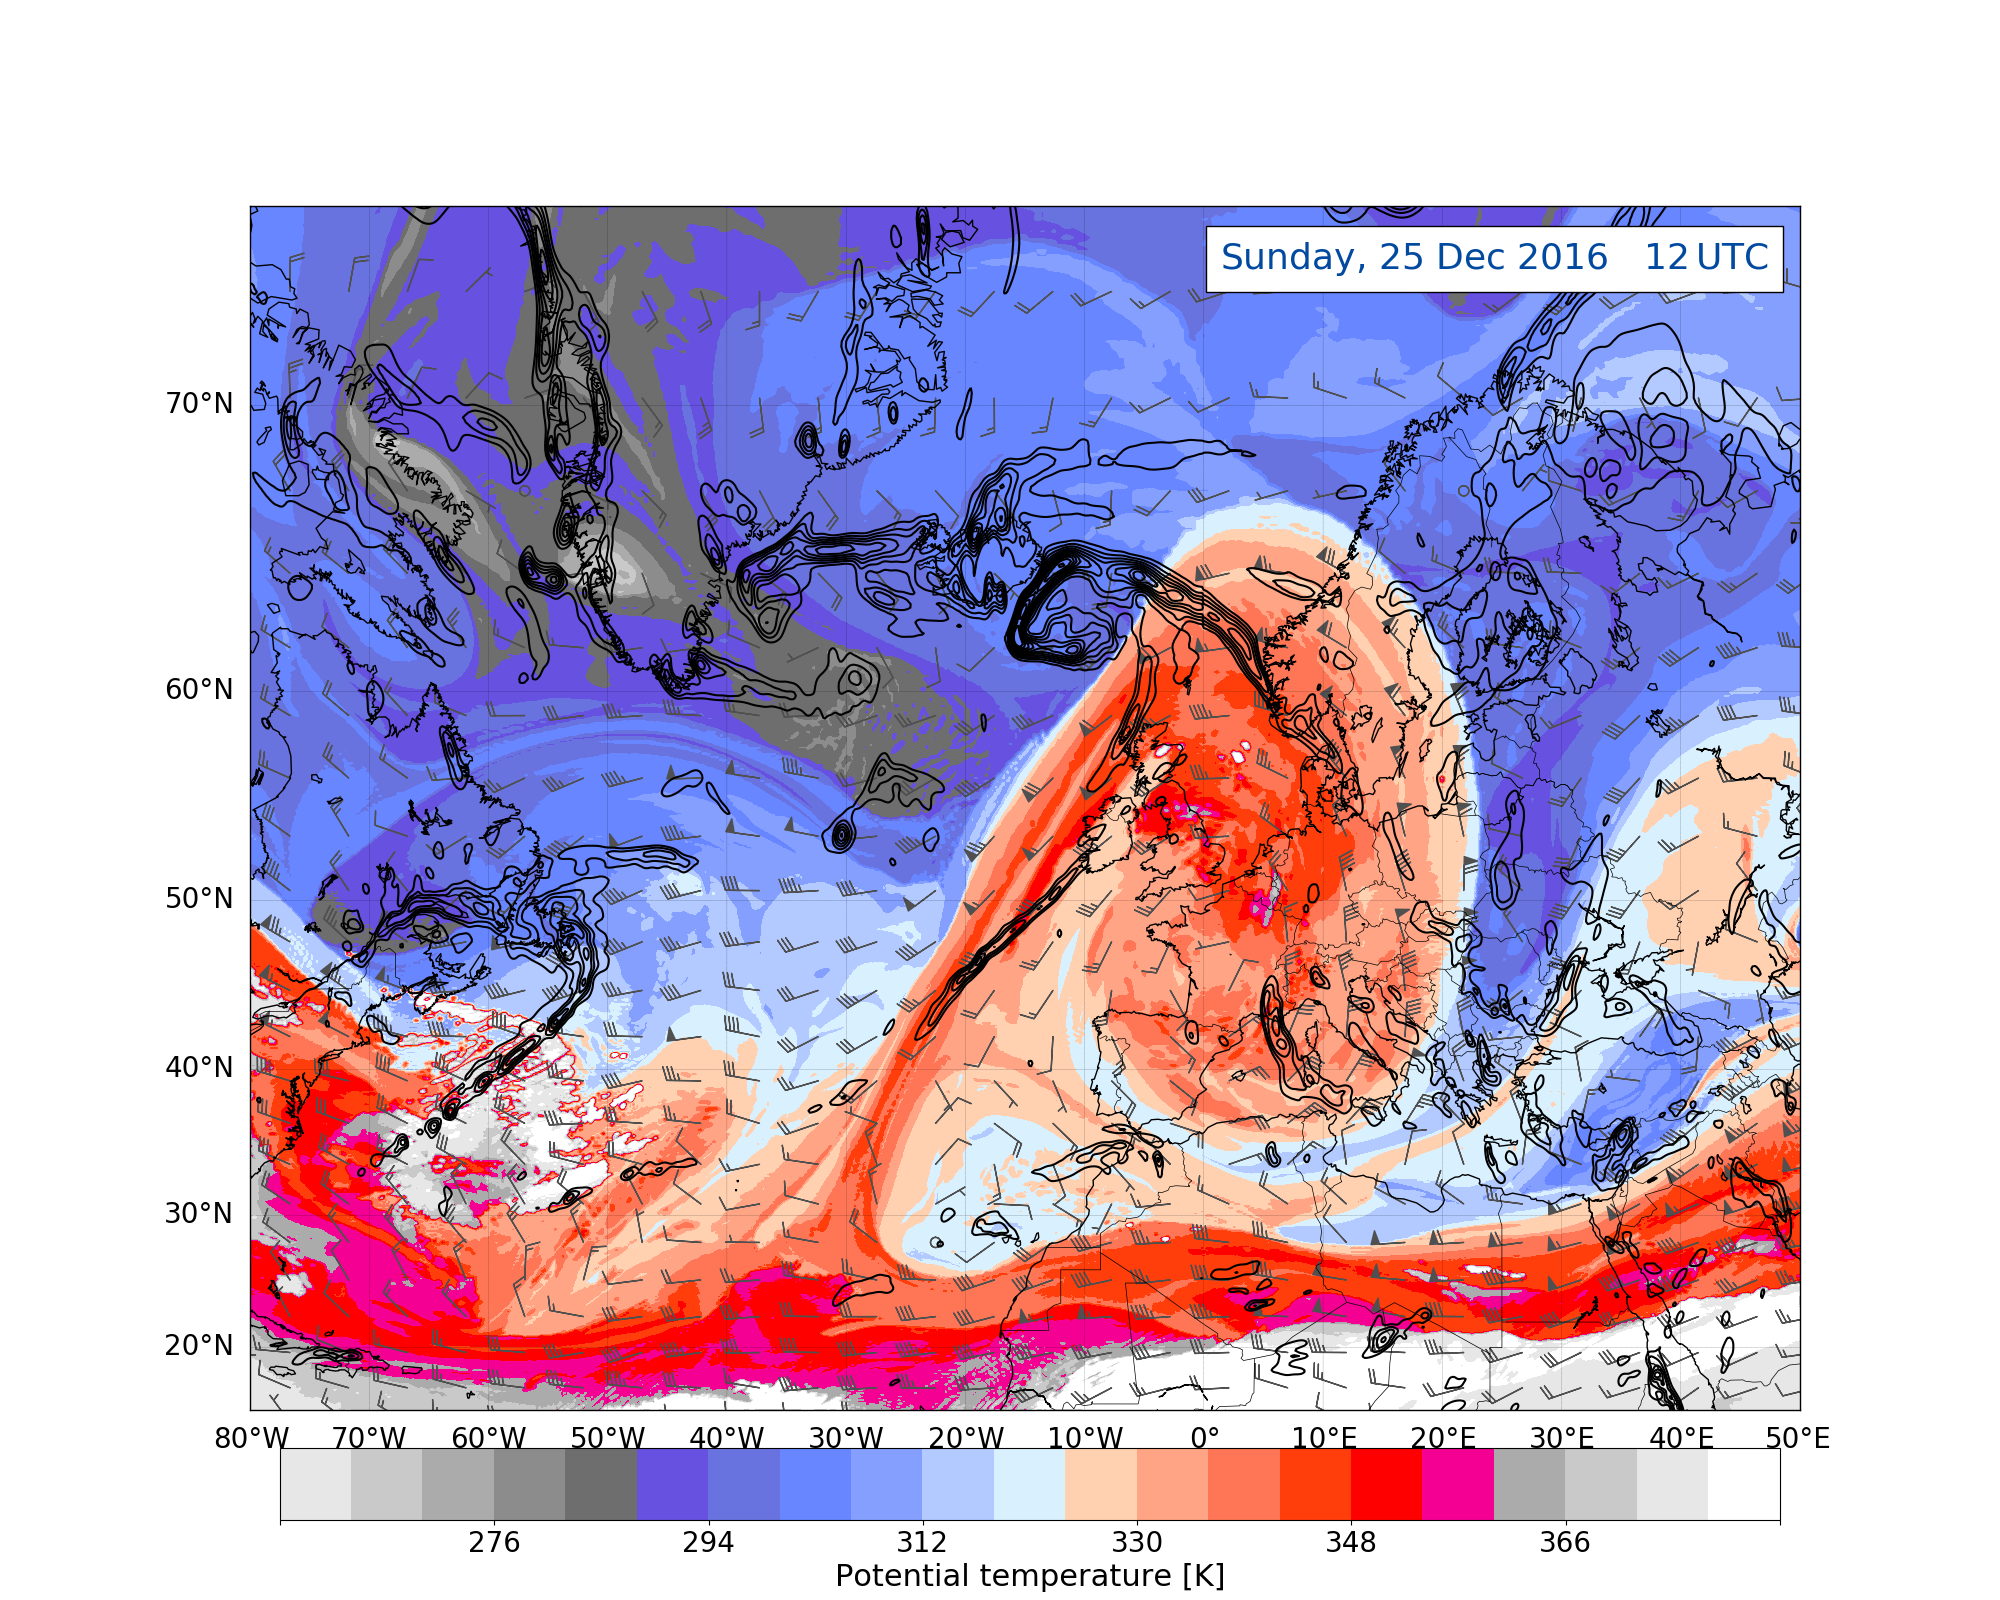
\includegraphics[trim={4.2cm 3.9cm 4.3cm 5.1cm},clip,
        width=\textwidth]{./fig_DynTropo/20161225_12}
        \caption{}\label{fig:DT25}
    \end{subfigure}    
%%%%%% 26/12
    \begin{subfigure}[b]{0.49\textwidth}
        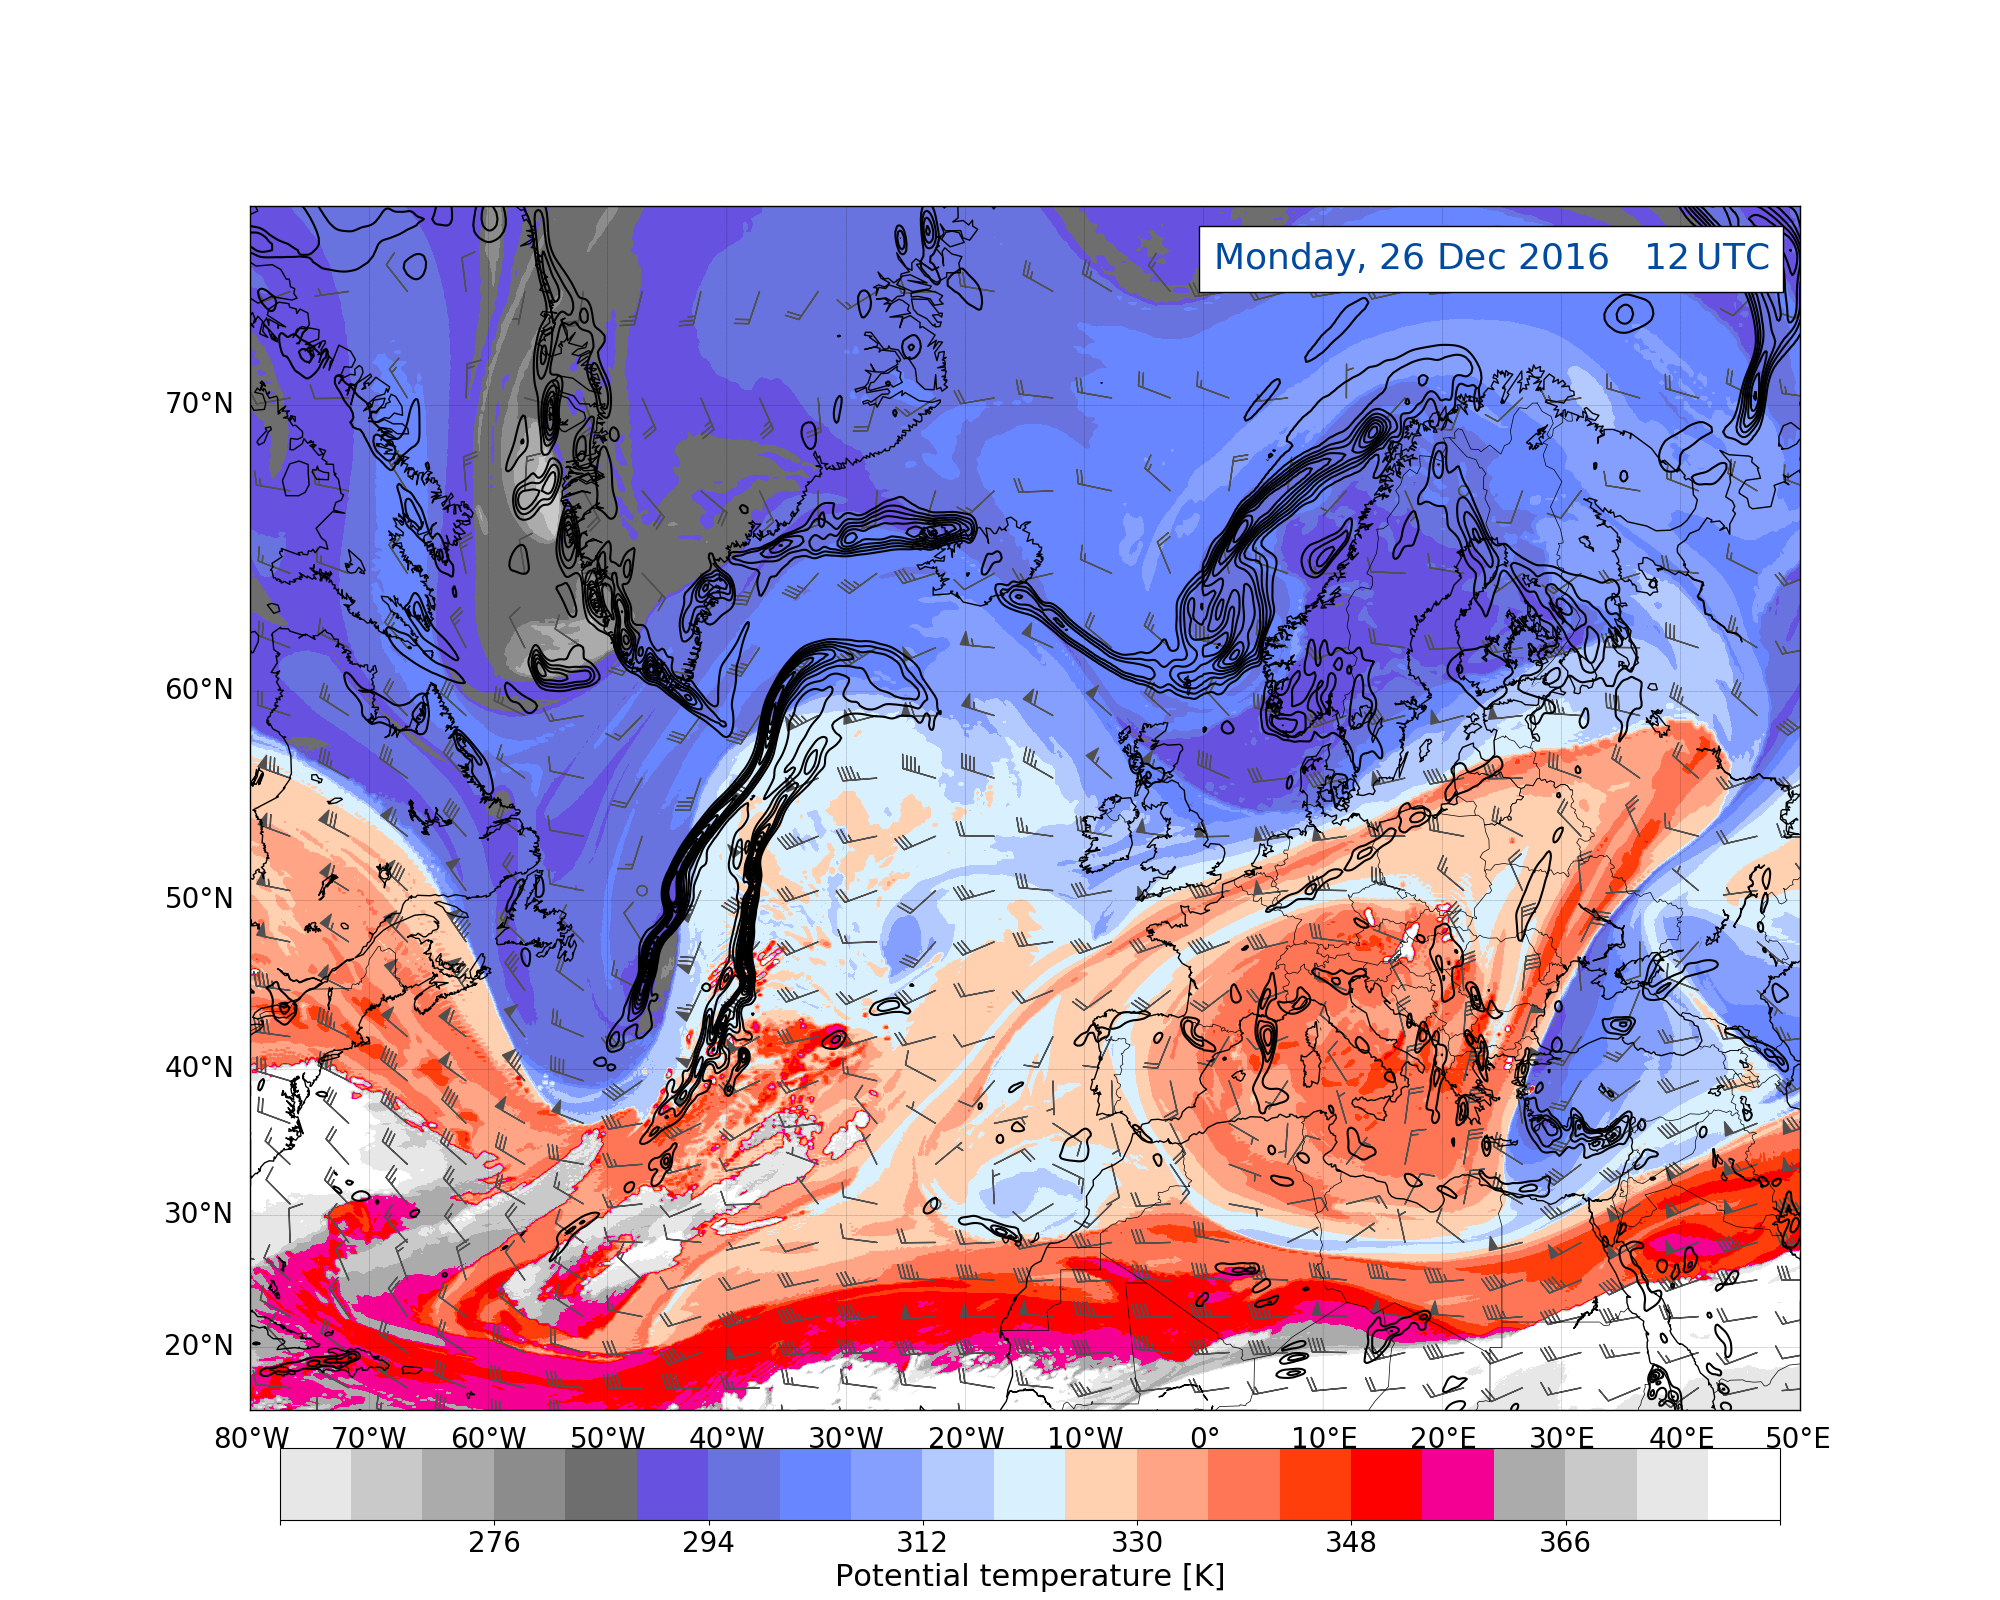
\includegraphics[trim={4.2cm 3.9cm 4.3cm 5.1cm},clip,
        width=\textwidth]{./fig_DynTropo/20161226_12}
        \caption{}\label{fig:DT26}
    \end{subfigure}
%%%%%% 27/12
    \begin{subfigure}[b]{0.49\textwidth}
        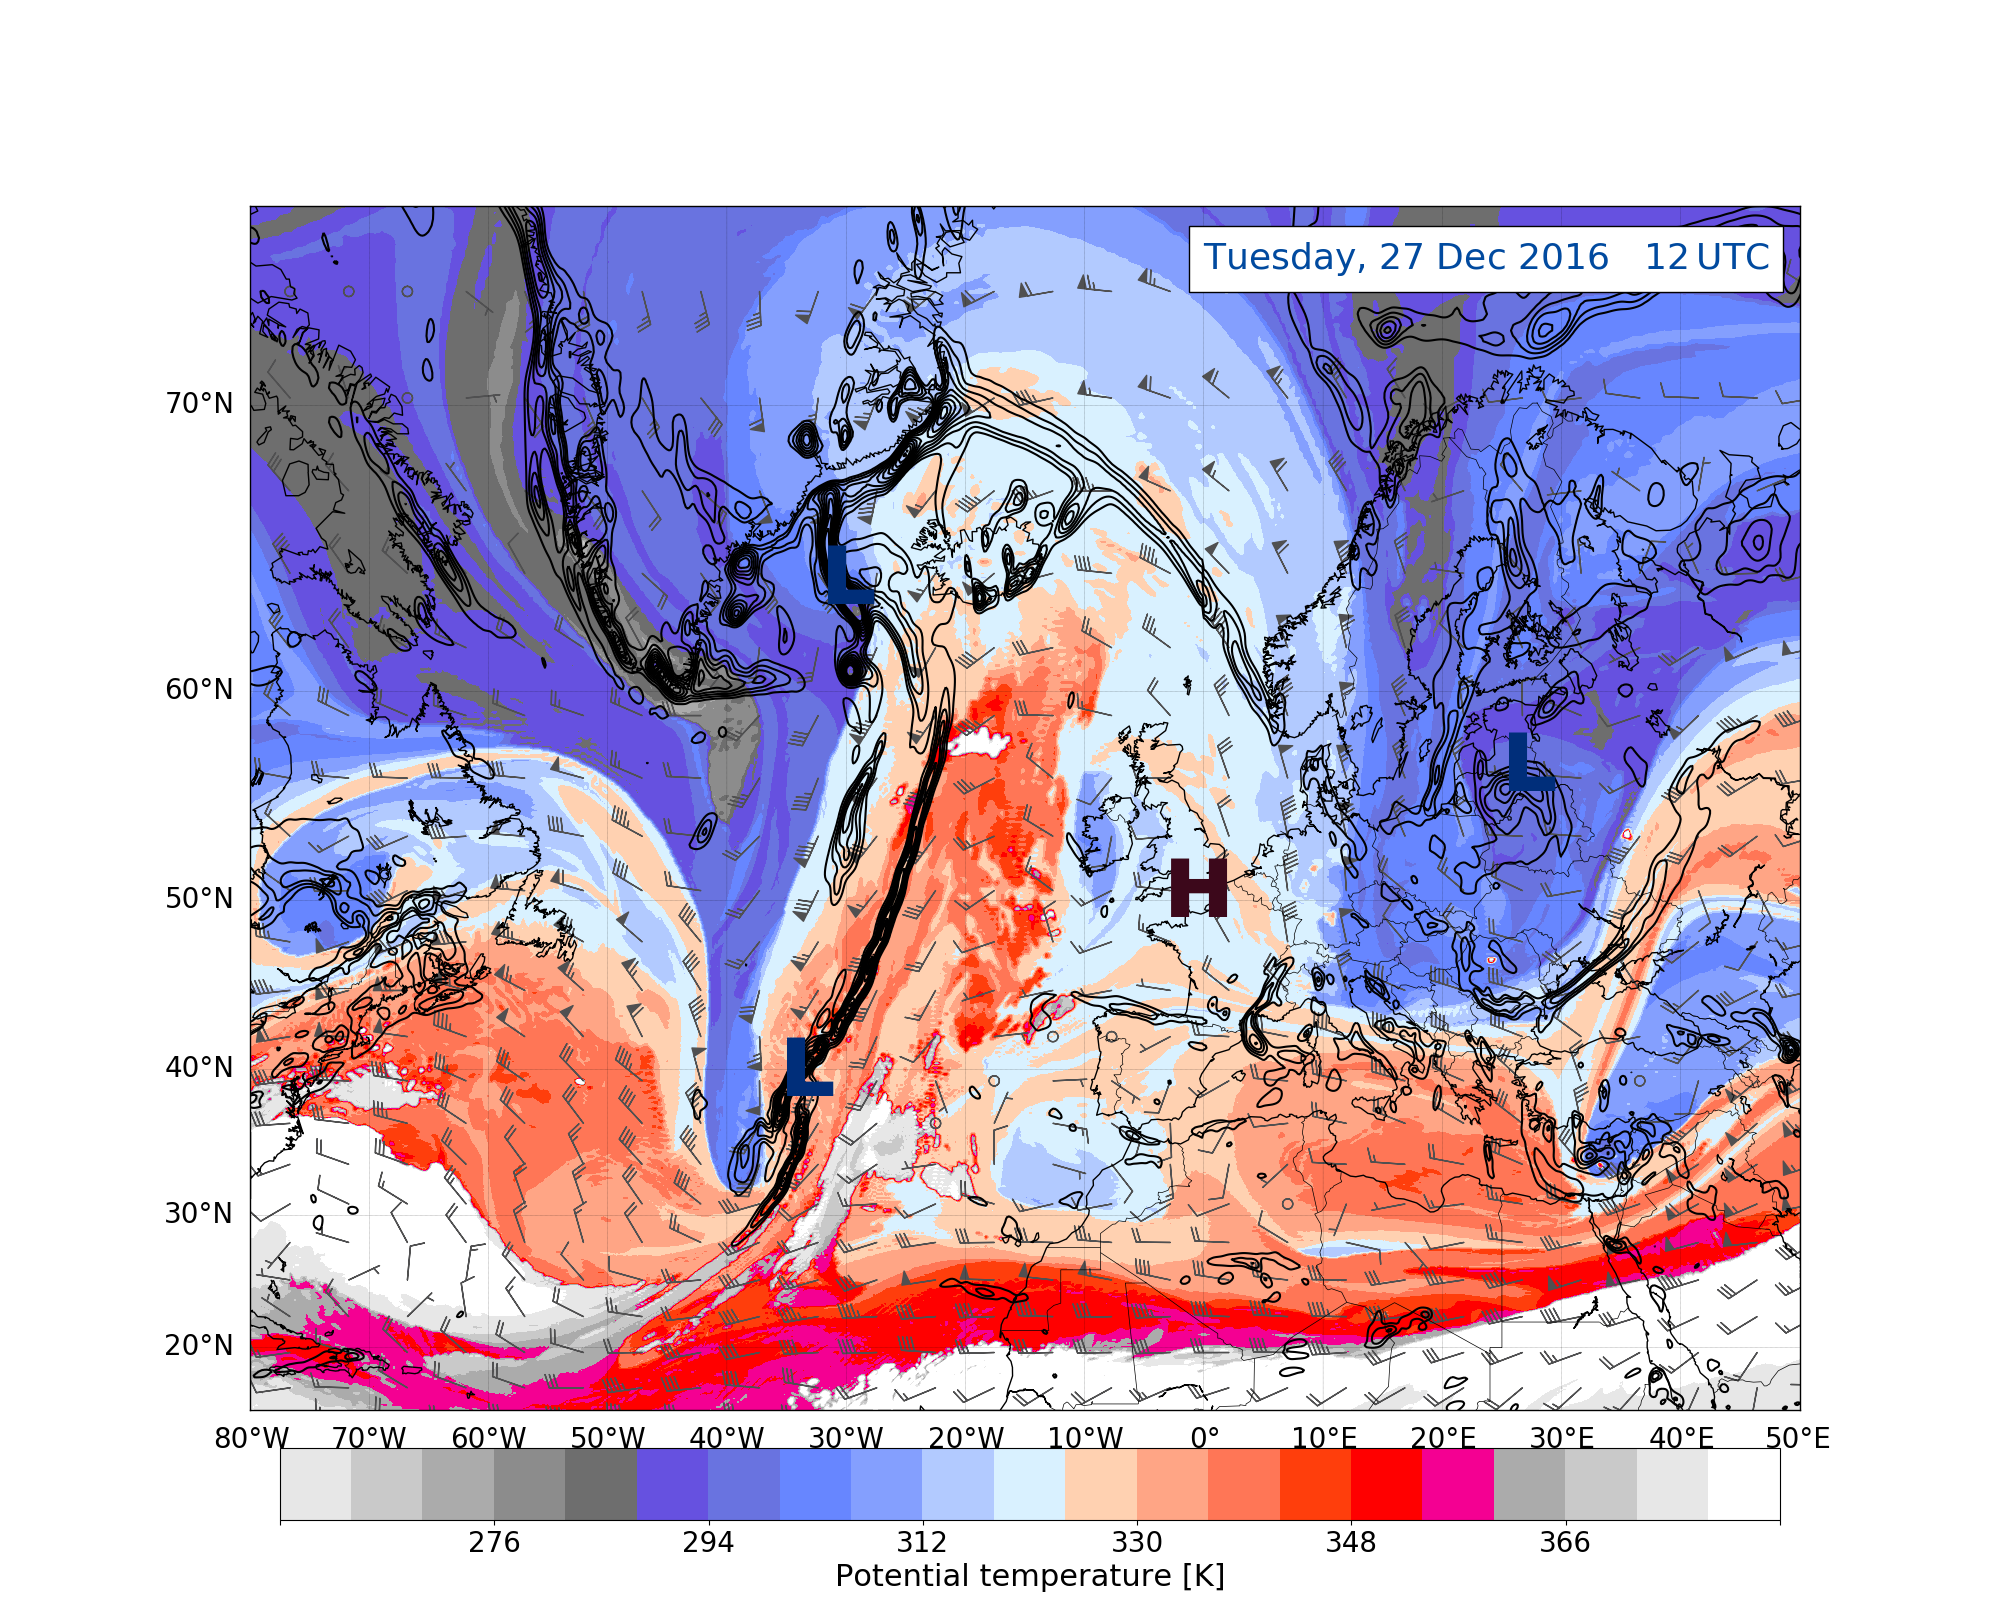
\includegraphics[trim={4.2cm 3.9cm 4.3cm 5.1cm},clip,
        width=\textwidth]{./fig_DynTropo/20161227_12}
        \caption{}\label{fig:DT27}
    \end{subfigure}   
%%%%%% label
    \begin{subfigure}[b]{\textwidth}
        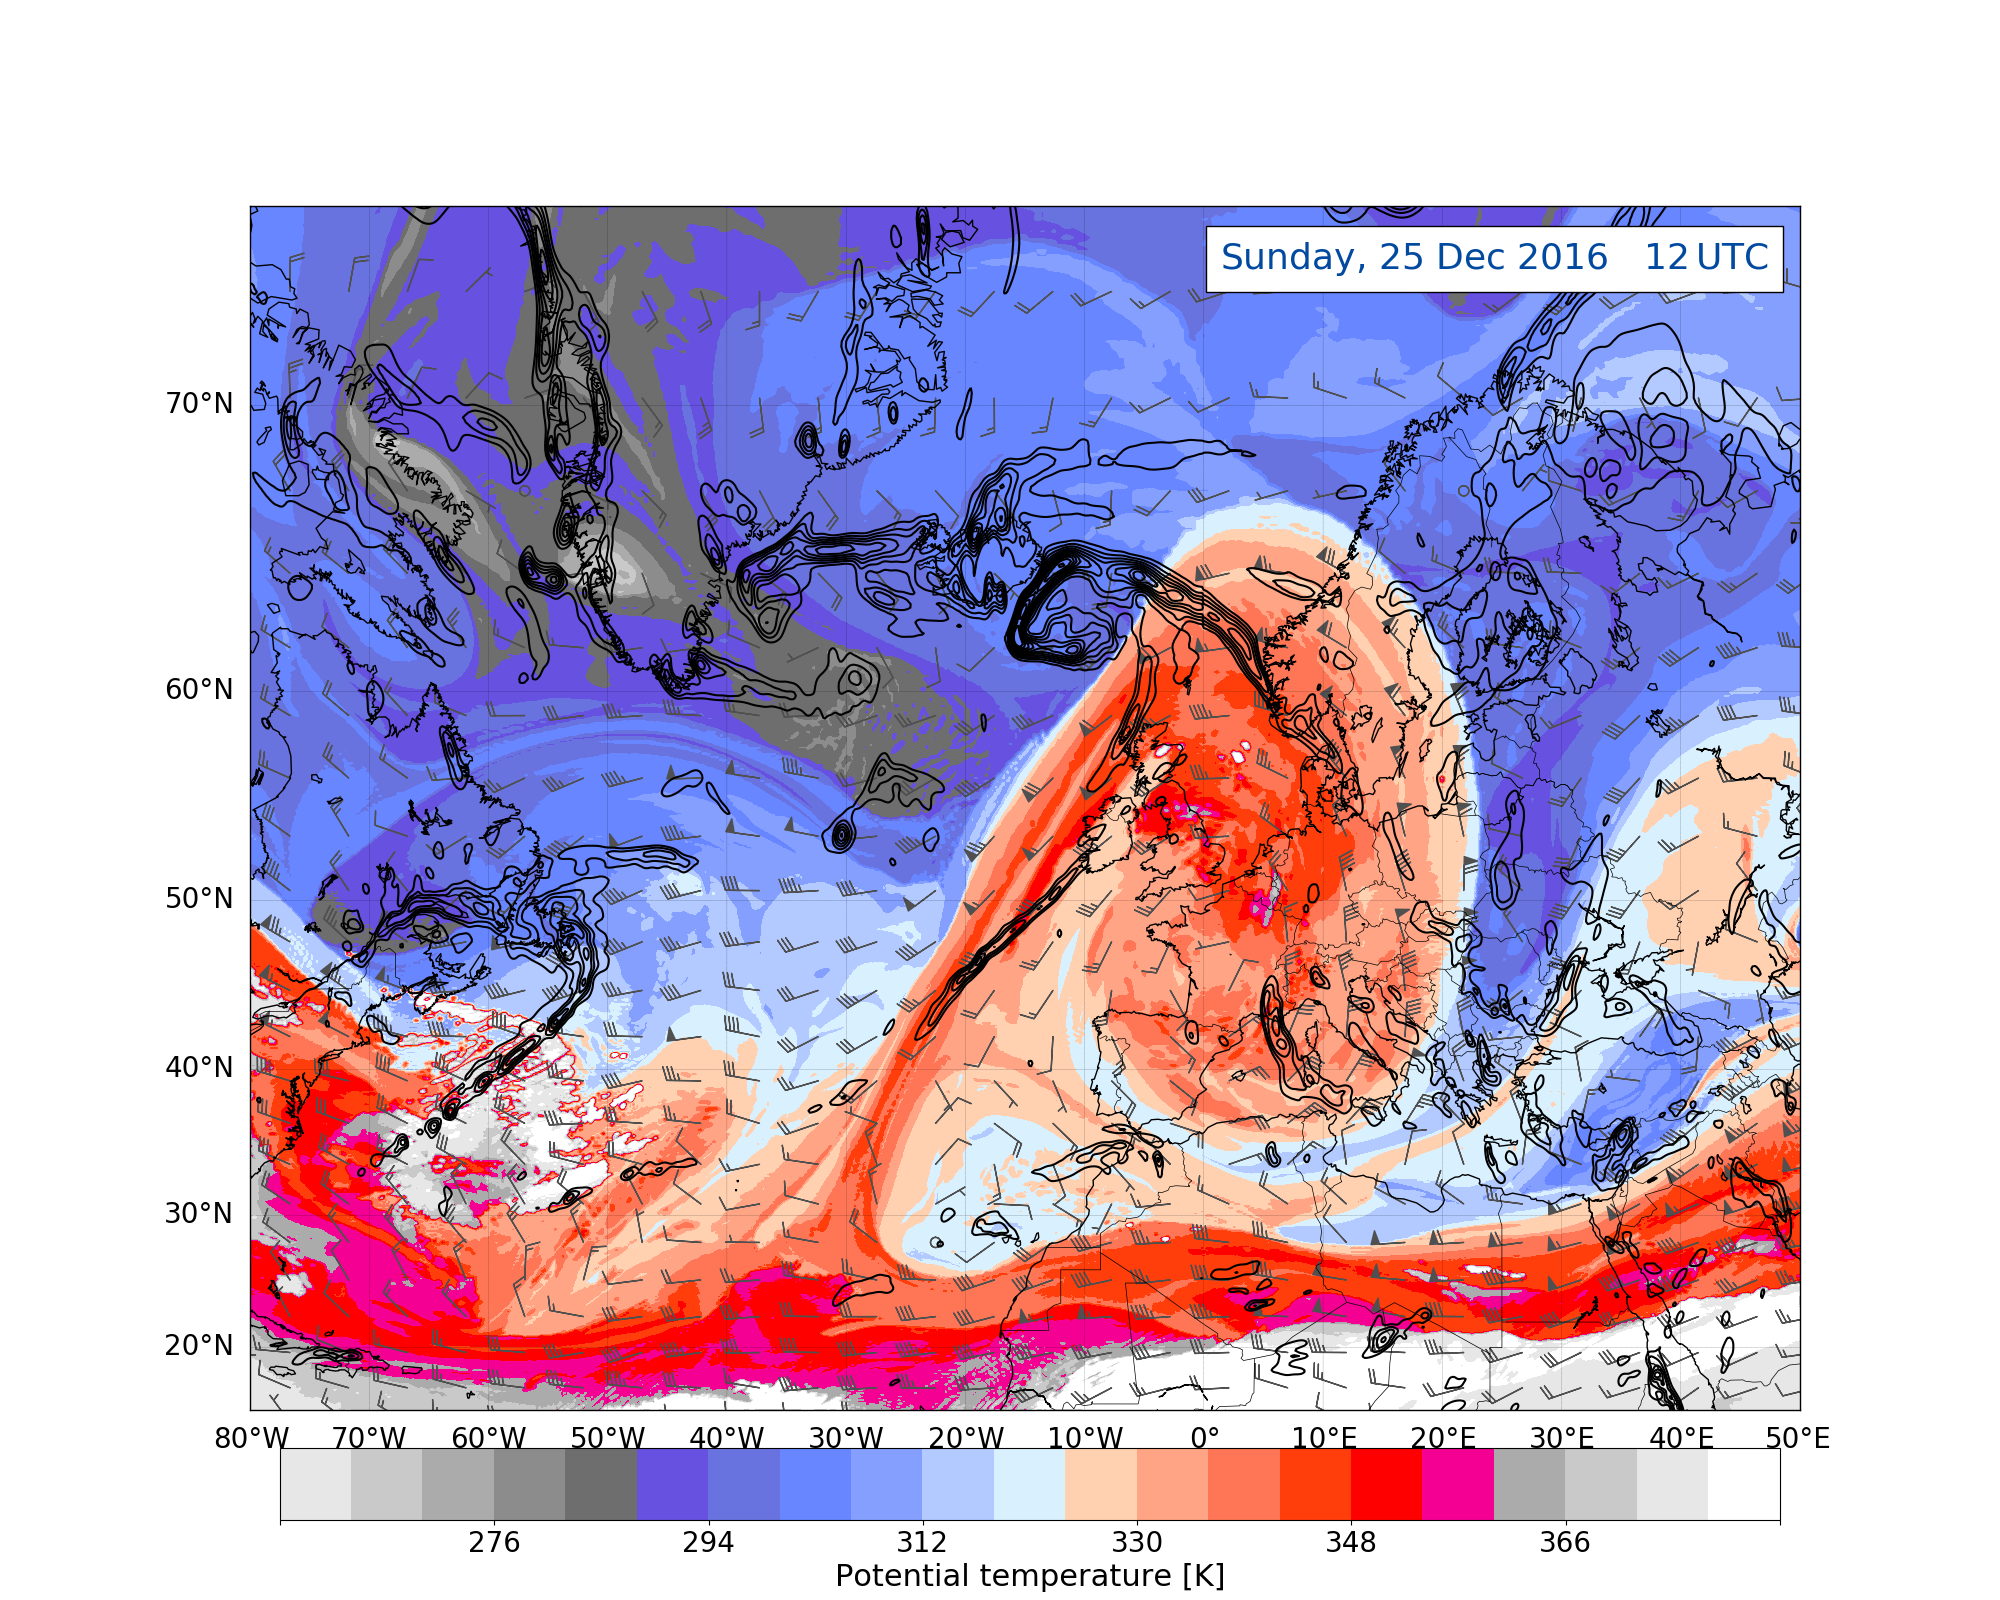
\includegraphics[trim={4.2cm 0cm 4.3cm 36.8cm},clip,
        width=\textwidth]{./fig_DynTropo/20161225_12}
    \end{subfigure}
    \caption{Dynamic tropopause analysis map, data from ECMWF at \SI{2}{PVU}. During \SIrange{20}{27}{\dec}. Potential temperature [K] at the \SI{2}{PVU} surface, shaded according to the colour bar. Total wind, barbs [\SI{}{\mPs}], and \SI{925}-\SI{850}{\hPa} layer-averaged surface relative vorticity (black contours, every \SI{.5e-4}{\per\second}).  }\label{fig:DynTropo}
\end{figure}
% %%%%%%%%%%%%%%%%%%%%%%%%%%%%%%%%%%%%%%%%%%%%%%%%%%%%%%%%%%%%%%%%%%%%%%%%%%
